\documentclass[lettersize,journal]{IEEEtran}
\usepackage{amsmath,amsfonts}
\usepackage{algorithmic}
\usepackage{algorithm}
\usepackage{array}
\usepackage[caption=false,font=normalsize,labelfont=sf,textfont=sf]{subfig}
\usepackage{textcomp}
\usepackage{stfloats}
\usepackage{url}
\usepackage{verbatim}
\usepackage{graphicx}
\usepackage{cite}
\usepackage[hidelinks]{hyperref}
\hyphenation{op-tical net-works semi-conduc-tor IEEE-Xplore}
% Prevent widow and orphan lines at column and page boundaries.
\widowpenalty=10000
\clubpenalty=10000
\displaywidowpenalty=10000
\brokenpenalty=10000
% updated with editorial comments 8/9/2021

% 自定义 Input 和 Output 命令
\makeatletter
\newcommand{\Input}{\item[\textbf{Input:}]}
\newcommand{\Output}{\item[\textbf{Output:}]}
\makeatother

\begin{document}

\title{A Compressive Sensing-Enhanced Ensemble Bayesian Optimization Algorithm for Expensive Black-Box Optimization}

\author{Fuqing Zhao, Xiaohuan Dong, Ling Wang,~\IEEEmembership{Senior Member,~IEEE,}and Hongyan Sang,~\IEEEmembership{Member,~IEEE}
        % <-this % stops a space
\thanks{This paper was produced by the IEEE Publication Technology Group. They are in Piscataway, NJ.}% <-this % stops a space
\thanks{Manuscript received April 19, 2021; revised August 16, 2021.}}

% The paper headers
\markboth{Journal of \LaTeX\ Class Files,~Vol.~14, No.~8, August~2021}%
{Shell \MakeLowercase{\textit{et al.}}: A Sample Article Using IEEEtran.cls for IEEE Journals}

\maketitle

\begin{abstract}
Global optimization of black-box functions characterized by unavailable closed-form expressions and derivatives, costly evaluations, and noisy observations arises in several engineering and scientific applications. Bayesian optimization (BO) with Gaussian process (GP) surrogates is sample efficient. However, stationary GP priors struggle to represent highly nonstationary and oscillatory objective functions. This limitation impairs global-structure reconstruction and acquisition decisions under tight evaluation budgets. Among compressive sensing (CS) formulations, Bayesian compressive sensing (BCS) is adopted because its posterior inference is compatible with the probabilistic structure of BO and provides the uncertainty estimates required for probabilistic surrogate modeling and acquisition design. Accordingly, \emph{BCS-Enhanced Ensemble Bayesian Optimization} (BCS-EEBO) is proposed as a two-level framework. At the surrogate level, a BCS-induced predictor is constructed using a sparse representation in a truncated discrete cosine transform (DCT) basis. The associated posterior uncertainty is quantified, and the resulting predictor is fused with a GP surrogate fitted to the observed data using an uncertainty-aware Gaussian fusion rule. At the acquisition level, expected improvement (EI) is combined with a BCS-based exploration score derived from the dominant uncertainty direction of the BCS posterior covariance. Experiments on benchmark functions and illustrative global-modeling tasks demonstrate that BCS-EEBO improves global reconstruction under sparse sampling and achieves superior optimization performance relative to the comparison methods under the same evaluation budgets. Ablation studies further demonstrate that surrogate-level and acquisition-level fusion make complementary contributions to the observed~improvements.
\end{abstract}

\begin{IEEEkeywords}
Bayesian optimization, Bayesian compressive sensing, ensemble surrogate modeling, acquisition function fusion, non-stationary optimization, expensive black-box optimization.
\end{IEEEkeywords}

\section{Introduction}
\IEEEPARstart{T}{he} global optimization of black-box functions---where closed-form expressions and derivatives are unavailable---arises broadly in engineering and scientific applications. Typical examples include neural architecture and hyperparameter tuning, reinforcement learning policy search \cite{Calandra2016GaitsBO}, simulation-based calibration to real-world data, and chemical engineering and materials discovery via high-throughput screening \cite{HernandezLobato2017PDTS}. In these settings, objective evaluations are often expensive and corrupted by stochastic noise, which makes evaluation-efficient optimization essential.

Gradient-free metaheuristics such as genetic algorithms \cite{Holland1975GA}, ant colony optimization \cite{Dorigo1996AntSystem}, and particle swarm optimization \cite{EberhartKennedy1995PSO} require only function values and impose minimal assumptions on the objective. However, they typically require many function evaluations, which becomes prohibitive when each evaluation is costly. Bayesian optimization (BO) addresses this challenge by fitting a probabilistic surrogate to previously evaluated samples and selecting new points with an acquisition function that balances exploration and exploitation \cite{Shahriari2016ReviewBO,Frazier2018TutorialBO}.

Standard Gaussian process (GP)-based BO often loses accuracy in highly nonlinear and non-stationary engineering systems. In many implementations, GPs use stationary kernels and simple mean functions. Under these priors, predictions far from observations tend to revert to the prior mean with increasing uncertainty, which limits extrapolation and global trend estimation unless more expressive kernel structures are adopted \cite{RasmussenWilliams2006GPML,WilsonAdams2013Kernels}. Stationary kernels also assume translation-invariant covariance; under non-stationarity, the resulting model mismatch reduces predictive fidelity and acquisition quality. Snoek et al.\ \cite{Snoek2014InputWarping} addressed this mismatch through input warping.

To address these limitations, Bayesian compressive sensing (BCS) is integrated with BO in the proposed \emph{BCS-Enhanced Ensemble Bayesian Optimization} (BCS-EEBO) framework. Among compressive sensing (CS) formulations, BCS is adopted because its posterior formulation is consistent with the Bayesian inference mechanism of BO and provides the uncertainty information required for surrogate fusion and acquisition-function design. Unlike conventional optimization-based CS formulations that primarily produce point estimates of sparse coefficients, BCS yields a posterior distribution that supports both response reconstruction and predictive uncertainty quantification \cite{JiXueCarin2008BCS}. BCS-based surrogates have also been applied to highly non-stationary responses with limited samples in engineering reliability analysis \cite{LiWang2022ABCSMCS}. In BCS-EEBO, scarce observations are processed through a modified BCS projection scheme, and the resulting surrogate is combined with GP-based BO so that their different modeling assumptions provide complementary information.

The main contributions are as follows:
\begin{enumerate}
  \item A modified-projection BCS method is developed for function modeling and uncertainty quantification in data-scarce settings.
  \item An ensemble BO scheme is designed to combine the global structure captured by the BCS surrogate with the local adaptation of GP-based modeling.
  \item An eigendecomposition-based criterion derived from the BCS posterior covariance is introduced to guide query selection.
\end{enumerate}

The remainder of this paper is organized as follows. Section~\ref{sec:literature} reviews surrogate models, ensemble BO methods, and BCS. Section~\ref{sec:method} presents the BCS-EEBO framework, including its BO and BCS modules, two-level fusion strategy, and algorithmic procedure. Section~\ref{sec:experiments} reports the experimental settings, comparative results, nonparametric statistical analysis, and ablation studies. Section~\ref{sec:conclusion} concludes the paper and outlines directions for future work.

\section{Literature Review}
\label{sec:literature}
\subsection{Surrogate Model}
In expensive black-box optimization, the objective function is typically unavailable in closed form and each evaluation is costly. Surrogate-based methods fit a computationally inexpensive approximation to limited observations and use it to select the next evaluation point. The choice of surrogate directly affects uncertainty quantification, the exploration--exploitation trade-off, and sample efficiency. Classical BO commonly adopts GPs, whose kernels encode input correlations and yield closed-form posterior predictive distributions \cite{RasmussenWilliams2006GPML,Shahriari2016ReviewBO,Frazier2018TutorialBO}. Tree-based surrogates are often preferable for mixed continuous and categorical variables, conditional hyperparameters, and nonsmooth piecewise objectives. For example, Sequential Model-based Algorithm Configuration uses random forests for algorithm configuration with conditional spaces \cite{Hutter2011SMAC}. The tree-structured Parzen estimator models conditional densities for hierarchical hyperparameter spaces \cite{bergstra2011algorithms}. Deep Gaussian processes increase modeling capacity by composing GP layers, at the cost of approximate inference and greater computation \cite{DamianouLawrence2013DeepGP,SalimbeniDeisenroth2017DSVI}. Deep kernel learning instead learns a neural representation before applying GP inference in the learned space \cite{Wilson2016DKL}. Bayesian additive regression trees provide posterior uncertainty and accommodate piecewise structure \cite{Chipman2010BART}. Bayesian neural networks and deep ensembles have also been investigated for higher-dimensional problems, although training cost and uncertainty calibration remain important \cite{Blundell2015WeightUncertainty,Lakshminarayanan2017DeepEnsembles}. The proposed method combines GP and BCS-based surrogate models to capture non-stationary global structure.

\subsection{Ensemble Method}
Ensemble methods reduce the sensitivity of BO to the surrogate family, kernel specification, and acquisition strategy. Existing approaches fall into two groups: (i) \emph{decision-level} ensembling, which aggregates recommendations from multiple models or acquisition strategies and forms ensemble Bayesian optimization (EBO); and (ii) \emph{prediction-level} ensembling, which combines posterior predictive distributions through Bayesian model averaging (BMA).

\textbf{(1) Decision-level ensembling.}
Decision-level EBO treats surrogate models or acquisition functions as a set of experts. Each expert proposes one or more candidate points, and an online rule aggregates the proposals. \textsc{GP-Hedge} formulates acquisition-function selection as a multi-armed bandit problem and applies the Hedge algorithm to adapt the acquisition weights over successive iterations \cite{Hoffman2011GPHedge}. The entropy search portfolio uses information-theoretic criteria to reduce sensitivity to noisy short-term rewards \cite{Shahriari2014ESP}. Methods that down-weight outdated performance signals \cite{Vasconcelos2019NoPAStBO} or tune portfolio hyperparameters through Thompson sampling \cite{Vasconcelos2022SETUPBO} further reduce sensitivity to the combination rule. For large-scale and high-dimensional problems, ensembles of additive GP models have been combined with batch acquisition and randomized divide-and-conquer procedures \cite{Wang2018EBO}. Ensemble Mashups jointly combines models and acquisition functions \cite{Ravishankar2024EnsembleMashups}. In warm-start and transfer settings, a ranking-weighted Gaussian process ensemble fits one GP to each source task and combines them through ranking-based weights \cite{Feurer2018RGPE}. Expected improvement (EI) is then applied to the resulting GP-form ensemble. Prior-robust decision rules have also been developed to reduce sensitivity to imprecise priors \cite{Rodemann2024ImpreciseBO}.

Decision-level EBO accommodates heterogeneous surrogates and acquisition strategies. Its combination rules, however, are often heuristic or based on online learning rather than posterior model probabilities. The resulting uncertainty estimates are therefore often less calibrated, and statistical optimality guarantees are difficult to establish \cite{Hoeting1999BMA}.

\textbf{(2) Prediction-level ensembling.}
In contrast to decision-level aggregation, BMA combines models at the level of the \emph{posterior predictive distribution} rather than aggregating acquisition values or candidate points. Given a model class $\{M_m\}$, BMA forms the predictive distribution as
\begin{equation}
p(y \mid x, \mathcal{D}) \;=\; \sum_{m} p(y \mid x, \mathcal{D}, M_m)\, p(M_m \mid \mathcal{D}),
\end{equation}
thereby integrating model uncertainty and reducing the overconfidence associated with selecting a single model \cite{Hoeting1999BMA}. Seeger \cite{Seeger2000BayesianModelSelection} studied Bayesian model selection for kernel-based learners through approximate inference. In BO, marginalization over GP hyperparameters improves uncertainty quantification \cite{Snoek2012PracticalBO}, and its effect under different noise and acquisition settings has been examined empirically \cite{DeAth2021HowBayesian}. Discrete kernel mixtures have been studied for Kriging-based optimization \cite{Ginsbourger2008DiscreteKernelMixtures}, and BMA has been applied to multi-kernel GP regression \cite{Yu2013BMAMKGPR}. Dirichlet process mixtures of GPs provide a more flexible alternative for spatially heterogeneous responses by identifying local regimes during optimization \cite{Zhang2026RAMBO}.

\subsection{Bayesian Compressive Sensing}
Compressed sensing assumes that a high-dimensional signal has a sparse or compressible representation in a suitable transform domain, such as a Fourier or discrete cosine basis, a wavelet basis, or an overcomplete dictionary. Under suitable conditions, stable reconstruction requires substantially fewer linear measurements than the ambient signal dimension. Cand\`es, Romberg, and Tao established recovery conditions for incomplete measurements \cite{CandesRombergTao2006RUP}, Cand\`es and Tao derived near-optimal guarantees for random projections \cite{CandesTao2006NearOptimal}, and Donoho summarized sparse-recovery theory \cite{Donoho2006CompressedSensing}.

Unlike non-Bayesian sparse recovery methods, including $\ell_1$-norm minimization and orthogonal matching pursuit, BCS and sparse Bayesian learning (SBL) estimate a posterior distribution over sparse coefficients. Their posterior means and covariances provide both a reconstruction and its uncertainty. This approach is closely related to the relevance vector machine (RVM) and automatic relevance determination (ARD). Tipping's sparse Bayesian learning framework assigns an independent prior-precision hyperparameter to each coefficient, which prunes unsupported basis functions \cite{Tipping2001RVM}. Wipf and Rao analyzed the corresponding basis-selection mechanism from a signal-processing perspective \cite{WipfRao2004BasisSelection}.

Ji, Xue, and Carin formulated BCS through joint inference over sparse coefficients and noise parameters \cite{JiXueCarin2008BCS}. The resulting posterior provides coefficient variances and credible intervals for adaptive sensing and sequential measurement design. Babacan, Molina, and Katsaggelos studied a Laplace-prior formulation and its trade-offs among sparsity, robustness, and inference \cite{Babacan2010LaplaceBCS}. Faul and Tipping analyzed marginal-likelihood optimization and the mechanism by which hyperparameter learning produces sparse solutions \cite{FaulTipping2001AnalysisSBL}. Extensions to multiple measurement vectors with shared sparsity were studied by Wipf and Rao \cite{WipfRao2007SimultaneousSparse}.

These studies establish that BCS and SBL provide posterior uncertainty together with sparse recovery \cite{Tipping2001RVM,WipfRao2004BasisSelection,JiXueCarin2008BCS}. The posterior covariance further guides sequential or adaptive sampling by propagating coefficient uncertainty through later inference and optimization \cite{JiXueCarin2008BCS}.

\section{BCS-Enhanced Ensemble Bayesian Optimization (BCS-EEBO)}
\label{sec:method}

The proposed BCS-EEBO method uses two-level fusion for expensive black-box global optimization. The following minimization problem is considered:
\begin{equation}
\label{eq:problem}
\min_{\mathbf{x}\in\mathcal{X}\subset\mathbb{R}^d} f(\mathbf{x}), \qquad
y = f(\mathbf{x}) + \epsilon,\ \ \epsilon\sim\mathcal{N}(0,\sigma_\epsilon^2),
\end{equation}
where $f$ is unknown, derivatives are unavailable, and evaluations are costly. BCS-EEBO integrates a standard GP-based BO loop with a BCS module. The GP surrogate fitted in the BO loop, denoted by BO-GP, represents local behavior near the observations. The BCS module uses a sparse transform-domain representation to estimate global and oscillatory structure together with transform-domain uncertainty. The two information sources are fused at the surrogate and acquisition levels.

\subsection{Notation and Candidate Set}
\label{subsec:notation}

At iteration $t$, the evaluated dataset is
\begin{equation}
\mathcal{D}_t=\{(\mathbf{x}_i,y_i)\}_{i=1}^{n_t}.
\end{equation}
For acquisition maximization, a finite candidate set $\mathcal{C}\subset\mathcal{X}$ (e.g., a dense grid or a Sobol set) is used, and the next query is selected by
\begin{equation}
\label{eq:next}
\mathbf{x}_{t+1} = \arg\max_{\mathbf{x}\in\mathcal{C}} a(\mathbf{x}).
\end{equation}
Let $\Omega_t\subset\mathcal{C}$ denote the index set of already-evaluated candidates (``known points'').

\subsection{Overall Framework}
\label{subsec:overall_framework}

BCS-EEBO follows the sequential model-based optimization (SMBO) framework \cite{bergstra2011algorithms}. As illustrated in Fig.~\ref{fig:framework}, each iteration contains four modules:

\begin{figure}[htbp]
    \centering
    % Adjust the width to scale the image.
    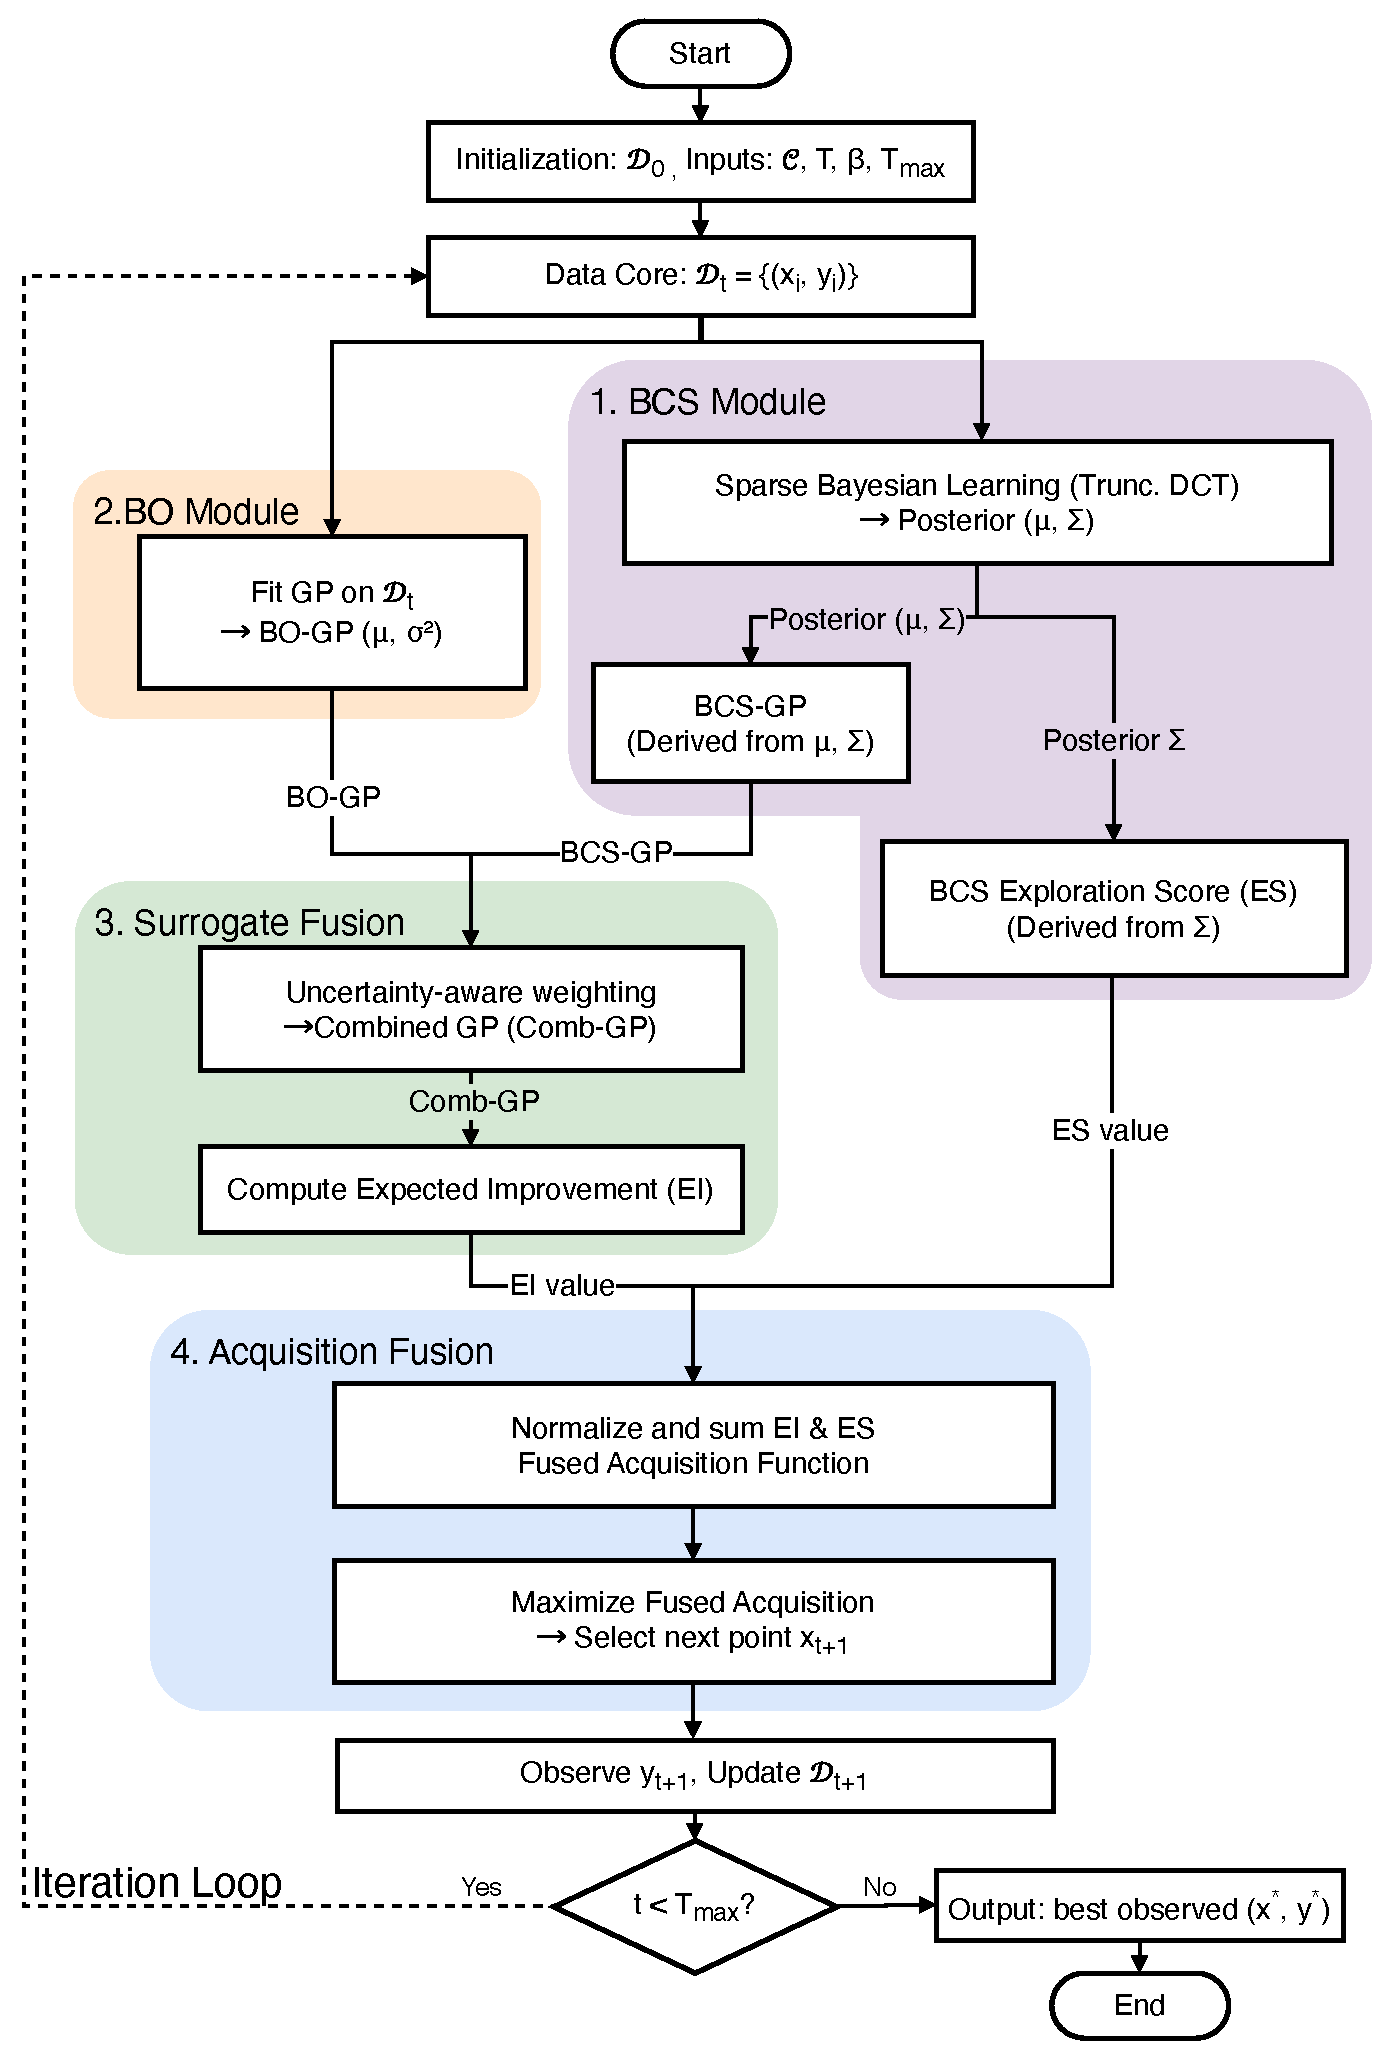
\includegraphics[width=0.98\linewidth]{farmekimi.drawio.pdf}
    \caption{The overall framework of the proposed BCS-EEBO algorithm.}
    \label{fig:framework}
\end{figure}

\begin{itemize}
    \item \textbf{1. BO Module:} A GP is fitted to $\mathcal{D}_t$ to represent local behavior of the objective function \cite{Jones1998EGO,Snoek2012PracticalBO,Shahriari2016ReviewBO}. The resulting BO-GP is described by $(\mu_{\mathrm{BO}}(\cdot),\sigma^2_{\mathrm{BO}}(\cdot))$.
    
    \item \textbf{2. BCS Module:} In parallel, sparse Bayesian learning is applied to a truncated discrete cosine transform (DCT) representation of $\mathcal{D}_t$ through ARD and the RVM \cite{JiXueCarin2008BCS,Tipping2001RVM}. The posterior mean and covariance $(\boldsymbol{\mu},\mathbf{\Sigma})$ of the active transform coefficients produce two outputs: a time-domain BCS-induced GP (BCS-GP) and an exploration score derived from $\mathbf{\Sigma}$.

    \item \textbf{3. Surrogate Fusion:} The BO-GP and BCS-GP predictive distributions are combined through uncertainty-aware weights to form a combined GP (Comb-GP). EI is evaluated on this fused distribution and therefore reflects both local and global information.

    \item \textbf{4. Acquisition Fusion:} The dominant uncertainty direction of $\mathbf{\Sigma}$ is mapped to the input domain to obtain the BCS exploration score. The normalized EI and exploration scores are added with a weighting coefficient, and the maximizer of the fused acquisition determines $\mathbf{x}_{t+1}$.
\end{itemize}

After $\mathbf{x}_{t+1}$ is selected, the corresponding response $y_{t+1}$ is observed and the dataset is updated as $\mathcal{D}_{t+1}=\mathcal{D}_t\cup\{(\mathbf{x}_{t+1},y_{t+1})\}$. The procedure is repeated until the termination criterion is met.

\begin{algorithm}[t]
\caption{Generic Sequential Model-Based Optimization }
\label{alg:smbo}
\begin{algorithmic}[1]
% \textbf{Input:}{Objective function $f$, initial model $M_0$, budget $T$, selection strategy $S$}\\
% \textbf{Output:}{Set of evaluated points and observations $\mathcal{H}$}
\Input Objective function $f$, initial model $M_0$, budget $T$, selection strategy $S$
\Output Set of evaluated points and observations $\mathcal{H}$
\STATE $\mathcal{H} \leftarrow \emptyset$
\FOR{$t = 1$ \TO $T$}
    \STATE $\mathbf{x}^{\star} \leftarrow \arg\min_{\mathbf{x}\in\mathcal{X}} S(\mathbf{x}, M_{t-1})$
    \STATE Evaluate $f(\mathbf{x}^{\star})$ \COMMENT{Expensive step}
    \STATE $\mathcal{H} \leftarrow \mathcal{H}\ \cup\ \{(\mathbf{x}^{\star}, f(\mathbf{x}^{\star}))\}$
    \STATE Fit a new model $M_t$ to $\mathcal{H}$
\ENDFOR
\RETURN $\mathcal{H}$
\end{algorithmic}
\end{algorithm}

\subsection{BO Module: GP Surrogate with EI }
\label{subsec:bo}

BCS-EEBO follows the SMBO procedure in Algorithm~\ref{alg:smbo}: the surrogate is refitted to all collected data, and the next expensive query is selected by optimizing an acquisition function \cite{bergstra2011algorithms,Jones1998EGO,Shahriari2016ReviewBO}.

The objective $f$ is modeled by a GP fitted to $\mathcal{D}_t$:
\begin{equation}
\label{eq:bo_gp}
f(\mathbf{x})\mid \mathcal{D}_t \sim \mathcal{N}\!\bigl(\mu_{\mathrm{BO}}(\mathbf{x}),\,\sigma_{\mathrm{BO}}^2(\mathbf{x})\bigr).
\end{equation}
For minimization, EI at $\mathbf{x}$ is defined as
\begin{equation}
\label{eq:ei_def}
\mathrm{EI}_{\mathrm{BO}}(\mathbf{x})=
\mathbb{E}\!\left[\max\!\bigl(0, f^\star - f(\mathbf{x})\bigr)\mid \mathcal{D}_t\right],
\quad f^\star=\min_{i\le n_t} y_i.
\end{equation}
With Gaussian predictive distribution, EI admits a closed form:
\begin{equation}
\begin{aligned}
\label{eq:ei_closed}
\mathrm{EI}_{\mathrm{BO}}(\mathbf{x})
=
\bigl(f^\star-&\mu_{\mathrm{BO}}(\mathbf{x})\bigr)\Phi(\gamma(\mathbf{x}))
+
\sigma_{\mathrm{BO}}(\mathbf{x})\phi(\gamma(\mathbf{x})),\\
\gamma(\mathbf{x})&=
\frac{f^\star-\mu_{\mathrm{BO}}(\mathbf{x})}{\sigma_{\mathrm{BO}}(\mathbf{x})},
\end{aligned}
\end{equation}
where $\Phi(\cdot)$ and $\phi(\cdot)$ are the cumulative distribution function and probability density function of the standard normal distribution, respectively. The BO-GP is most informative in regions supported by nearby samples, while EI balances local improvement against predictive uncertainty.

\subsection{BCS Module: Sparse Transform-Domain Modeling with Uncertainty}
The BCS module follows the adaptive Bayesian compressive sensing formulation of Ji et al.\ \cite{JiXueCarin2008BCS}. A sparse DCT representation is used to model global non-stationary and oscillatory behavior, and its coefficient posterior quantifies uncertainty for both levels of fusion. Unlike static compressive sensing, the module refines the sparse representation and posterior uncertainty using the evaluated points at each iteration. It returns two outputs: (i) a BCS-GP for surrogate-level fusion and (ii) a transform-domain exploration score for acquisition-level fusion. Algorithm~\ref{alg:bcs_module} summarizes the procedure, and the following subsections provide its mathematical details.

\subsubsection{Overall Framework of the BCS Module}
The BCS module consists of four stages:
\begin{enumerate}
    \item \textbf{Stage 1: Truncated DCT dictionary construction}: A truncated DCT dictionary is constructed over $\mathcal{C}$. Low-frequency basis functions are retained to reduce dimensionality and improve numerical stability under sparse sampling.
    \item \textbf{Stage 2: Sparse Bayesian learning and effective-subspace identification}: A transform-domain linear model is fitted to $\mathcal{D}_t$ with the ARD prior in the RVM framework. The retained basis functions define a $K$-dimensional effective subspace with posterior mean $\mu$ and covariance $\Sigma$.
    \item \textbf{Stage 3: Two-phase adaptive optimization}: In Phase~1, a generalized Rayleigh quotient is solved under the known-point support constraint to identify a feasible, informative projection direction. A full-space projection complement is then applied to reduce bias from the initial RVM estimate. In Phase~2, the dominant uncertainty direction of the refined posterior covariance is mapped to the input domain to form the BCS exploration score.
    \item \textbf{Stage 4: Time-domain BCS-GP construction}: The posterior distribution of the active transform coefficients is mapped to the input domain, yielding the closed-form predictive mean and variance of the BCS-GP. This surrogate provides global and oscillatory information for fusion with the locally adaptive BO-GP.
\end{enumerate}

\begin{algorithm}[!t]
\caption{BCS Module with Adaptive Uncertainty Refinement}
\label{alg:bcs_module}
\begin{algorithmic}[1]
\Input Candidate set $\mathcal{C}$, dataset $\mathcal{D}_t$, known-point indices $\Omega_t$, DCT order $T$, RVM tolerance $\epsilon_{\mathrm{RVM}}$, Phase-1 tolerance $\epsilon_1$, maximum iterations $I_{\max,0}$ and $I_{\max,1}$, active-basis threshold $\alpha_{\max}=10^6$
\Output BCS-GP predictor $(\mu_{\mathrm{BCS}}(\cdot),\sigma_{\mathrm{BCS}}^2(\cdot))$, active-coefficient posterior $(\boldsymbol{\mu},\boldsymbol{\Sigma})$, and exploration score $g(\cdot)$

\STATE $\mathbf{B}\leftarrow\operatorname{TruncatedDCT}(\mathcal{C},T)$
\STATE $\mathbf{A}\leftarrow\mathbf{B}[\Omega_t,:]$, $\mathbf{y}\leftarrow[y_i]_{i\in\Omega_t}$

\STATE \textbf{RVM--ARD posterior estimation}
\STATE Initialize $\boldsymbol{\alpha}>0$, $\tau>0$, $q\leftarrow0$, and $\delta_{\mathrm{RVM}}\leftarrow+\infty$
\WHILE{$\delta_{\mathrm{RVM}}>\epsilon_{\mathrm{RVM}}$ AND $q<I_{\max,0}$}
    \STATE $\boldsymbol{\Sigma}_{\mathrm{full}}\leftarrow\left(\tau\mathbf{A}^T\mathbf{A}+\operatorname{diag}(\boldsymbol{\alpha})\right)^{-1}$
    \STATE $\boldsymbol{\mu}_{\mathrm{full}}\leftarrow\tau\boldsymbol{\Sigma}_{\mathrm{full}}\mathbf{A}^T\mathbf{y}$
    \STATE $\gamma_j\leftarrow1-\alpha_j\boldsymbol{\Sigma}_{\mathrm{full}}(j,j)$, $j=1,\ldots,T$
    \STATE $\alpha_j^{\mathrm{new}}\leftarrow\gamma_j/\mu_{\mathrm{full},j}^2$, $j=1,\ldots,T$
    \STATE $(\tau^{\mathrm{new}})^{-1}\leftarrow\|\mathbf{y}-\mathbf{A}\boldsymbol{\mu}_{\mathrm{full}}\|_2^2/(|\Omega_t|-\sum_{j=1}^{T}\gamma_j)$
    \STATE $\delta_{\mathrm{RVM}}\leftarrow\max\left\{\frac{\|\boldsymbol{\alpha}^{\mathrm{new}}-\boldsymbol{\alpha}\|_\infty}{\|\boldsymbol{\alpha}\|_\infty+10^{-12}},\frac{|\tau^{\mathrm{new}}-\tau|}{\tau+10^{-12}}\right\}$
    \STATE $\boldsymbol{\alpha}\leftarrow\boldsymbol{\alpha}^{\mathrm{new}}$, $\tau\leftarrow\tau^{\mathrm{new}}$, $q\leftarrow q+1$
\ENDWHILE
\STATE Recompute $\boldsymbol{\Sigma}_{\mathrm{full}}$ and $\boldsymbol{\mu}_{\mathrm{full}}$ using the converged $\boldsymbol{\alpha}$ and $\tau$
\STATE $\kappa\leftarrow\{j:\alpha_j<\alpha_{\max}\}$, $\mathbf{B}_a\leftarrow\mathbf{B}[:,\kappa]$
\STATE $\boldsymbol{\mu}\leftarrow\boldsymbol{\mu}_{\mathrm{full}}[\kappa]$, $\boldsymbol{\Sigma}\leftarrow\boldsymbol{\Sigma}_{\mathrm{full}}[\kappa,\kappa]$

\STATE \textbf{Known-point constrained projection refinement}
\STATE $iter\leftarrow0$, $\Delta\leftarrow+\infty$
\WHILE{$\Delta>\epsilon_1$ AND $iter<I_{\max,1}$}
    \STATE $\boldsymbol{\Sigma}_{\mathrm{old}}\leftarrow\boldsymbol{\Sigma}$, $\boldsymbol{\mu}_{\mathrm{old}}\leftarrow\boldsymbol{\mu}$
    \STATE $\mathbf{L}\leftarrow\mathbf{B}_a[\Omega_t,:]^T$
    \STATE Solve $(\mathbf{L}^T\boldsymbol{\Sigma}\mathbf{L})\mathbf{x}^*=\lambda_{\max}(\mathbf{L}^T\mathbf{L})\mathbf{x}^*$
    \STATE Normalize $\mathbf{x}^*$ such that $(\mathbf{x}^*)^T\mathbf{L}^T\mathbf{L}\mathbf{x}^*=1$
    \STATE $\mathbf{r}^*\leftarrow\mathbf{L}\mathbf{x}^*$
    \STATE $\boldsymbol{\Sigma}\leftarrow\left(\boldsymbol{\Sigma}_{\mathrm{old}}^{-1}+\tau\mathbf{r}^*(\mathbf{r}^*)^T\right)^{-1}$
    \STATE $\boldsymbol{\mu}\leftarrow\boldsymbol{\Sigma}\left(\boldsymbol{\Sigma}_{\mathrm{old}}^{-1}\boldsymbol{\mu}_{\mathrm{old}}+\tau\mathbf{r}^*(\mathbf{r}^*)^T\boldsymbol{\mu}_{\mathrm{old}}\right)$
    \STATE $(\kappa,\boldsymbol{\mu},\boldsymbol{\Sigma})\leftarrow\operatorname{ProjectionComplement}(\kappa,\boldsymbol{\mu},\boldsymbol{\Sigma})$
    \STATE $\mathbf{B}_a\leftarrow\mathbf{B}[:,\kappa]$
    \STATE $\Delta\leftarrow|\operatorname{tr}(\boldsymbol{\Sigma})-\operatorname{tr}(\boldsymbol{\Sigma}_{\mathrm{old}})|/\operatorname{tr}(\boldsymbol{\Sigma}_{\mathrm{old}})$, $iter\leftarrow iter+1$
\ENDWHILE

\STATE \textbf{Exploration score and BCS-GP construction}
\STATE $(\lambda_{\max},\mathbf{v}_{\max})\leftarrow\operatorname{EigMax}(\boldsymbol{\Sigma})$
\STATE $\boldsymbol{\phi}(x)\leftarrow\mathbf{B}[\operatorname{idx}(x),\kappa]^T$
\STATE $g(x)\leftarrow|\boldsymbol{\phi}(x)^T\mathbf{v}_{\max}|$
\STATE $\mu_{\mathrm{BCS}}(x)\leftarrow\boldsymbol{\phi}(x)^T\boldsymbol{\mu}$
\STATE $\sigma_{\mathrm{BCS}}^2(x)\leftarrow\boldsymbol{\phi}(x)^T\boldsymbol{\Sigma}\boldsymbol{\phi}(x)$

\RETURN $(\mu_{\mathrm{BCS}}(\cdot),\sigma_{\mathrm{BCS}}^2(\cdot))$, $(\boldsymbol{\mu},\boldsymbol{\Sigma})$, $g(\cdot)$
\end{algorithmic}
\end{algorithm}

\subsubsection{Truncated DCT Dictionary Construction}
The objective values on $\mathcal{C}$ are represented by a vector $f \in \mathbb{R}^{|\mathcal{C}|}$ ordered by candidate index. BCS assumes that $f$ is sparse or compressible in the DCT domain; therefore, a small number of DCT basis functions with non-negligible coefficients approximate $f$. For a $d$-dimensional input space, a 1D DCT basis matrix is constructed for each dimension, and their tensor outer product forms the full-dimensional dictionary following Li et al.\ \cite{li2025efficient}.

For the $q$-th input dimension with discrete resolution $N_q$, the entry in row $i_n$ and column $j_n$ of the 1D DCT basis matrix $B^q \in \mathbb{R}^{N_q \times N_q}$ is defined as
\begin{equation}
B^q(i_n,j_n)
=c_{j_n}\cos\left(
\frac{\pi(j_n-1)(X_{i_n}^q-X_1^q)}{N_q\eta_q}
+\frac{j_n-1}{4N_q}
\right)
\end{equation}
where $c_{j_n} = \sqrt{1/N_q}$ if $j_n=1$, and $c_{j_n} = \sqrt{2/N_q}$ otherwise; $X_{i_n}^q$ denotes the $i_n$-th discrete value of the $q$-th input variable, and $\eta_q$ is the interpolation resolution of the $q$-th dimension. The full-dimensional DCT basis matrix $B_{full} \in \mathbb{R}^{|\mathcal{C}| \times |\mathcal{C}|}$ is constructed via the outer product of the 1D DCT bases:
\begin{equation}
B_{j_1,j_2,...,j_d} = b_{j_1}^1 \otimes b_{j_2}^2 \otimes \cdots \otimes b_{j_d}^d
\end{equation}
where $b_{j_q}^q$ is the $j_q$-th column of $B^q$, and $\otimes$ denotes the tensor outer product.

To reduce dimensionality and improve numerical stability under sparse sampling, only the first $T$ low-frequency columns of $B_{full}$ are retained:
\begin{equation}
f \approx B w, \quad B \in \mathbb{R}^{|\mathcal{C}| \times T}, \quad T \ll |\mathcal{C}|
\end{equation}
where $w \in \mathbb{R}^T$ is the truncated transform coefficient vector. Low-frequency DCT basis functions dominate the global structure and non-stationary trend of the objective function, while high-frequency components mainly capture local noise and fine-grained fluctuations that are difficult to infer from sparse samples. Truncation thus reduces the solution dimensionality, mitigates overfitting, and improves the robustness of subsequent sparse Bayesian learning.

\subsubsection{Linear Measurements and Sparse Bayesian Learning via RVM-ARD}
The rows of $B$ indexed by the known-point set $\Omega_t$, with $m=|\Omega_t|$, form the observation matrix $A \in \mathbb{R}^{m \times T}$. The observed values $y$ and transform coefficients $w$ satisfy the linear model
\begin{equation}
y = A w + \varepsilon, \quad \varepsilon \sim \mathcal{N}(0, \sigma^2 I)
\end{equation}
where $\varepsilon$ is the additive Gaussian observation noise with variance $\sigma^2$, and $\tau = 1/\sigma^2$ denotes the noise precision.

Sparse Bayesian learning is performed with the hierarchical ARD prior in the RVM framework \cite{Tipping2001RVM}, which underlies the BCS formulation \cite{JiXueCarin2008BCS}. Each truncated transform coefficient $w_j$ is assigned a zero-mean Gaussian prior with an independent precision hyperparameter $\alpha_j$:
\begin{equation}
p(w_j | \alpha_j) = \mathcal{N}(w_j | 0, \alpha_j^{-1}), \quad \alpha_j > 0
\end{equation}
The hyperparameter $\alpha_j$ controls the sparsity-inducing prior. As $\alpha_j \to +\infty$, the prior variance of $w_j$ approaches zero and the corresponding basis function is pruned. A non-informative Gamma prior is assigned to the noise precision $\tau$.

Given the observed data $y$, the posterior distribution of the transform coefficients $w$ is derived via Bayesian inference. Conditioned on the hyperparameters $\alpha$ and $\tau$, the posterior of $w$ follows a multivariate Gaussian distribution:
\begin{equation}
p(w | y, \alpha, \tau) = \mathcal{N}(\mu_{full}, \Sigma_{full})
\end{equation}
where the posterior mean and covariance are given by:
\begin{equation}
\Sigma_{full} = \left( \tau A^T A + \text{diag}(\alpha) \right)^{-1}, \quad \mu_{full} = \tau \Sigma_{full} A^T y
\end{equation}
The hyperparameters $\alpha$ and $\tau$ are optimized via Type-II maximum likelihood estimation (evidence maximization), which iteratively updates the hyperparameters to maximize the marginal likelihood of the observed data. The update rules for the hyperparameters are:
\begin{equation}
\alpha_j^{new} = \frac{\gamma_j}{\mu_{full,j}^2}, \quad \frac{1}{\tau^{new}} = \frac{\|y - A\mu_{full}\|_2^2}{m - \sum_{j=1}^T \gamma_j}
\end{equation}
where $\gamma_j = 1 - \alpha_j \Sigma_{full}(j,j)$ represents the well-determinedness of the $j$-th coefficient.

After convergence, coefficients satisfying $\alpha_j < 10^6$ are retained in the active index set $\kappa$, which defines a $K$-dimensional effective transform subspace. The active basis matrix, observation matrix, and coefficient vector are denoted by $B_a = B[:, \kappa] \in \mathbb{R}^{|\mathcal{C}| \times K}$, $A_a = A[:, \kappa] \in \mathbb{R}^{m \times K}$, and $w_\kappa \in \mathbb{R}^K$, respectively. Their posterior distribution is
\begin{equation}
p(w_\kappa | y) = \mathcal{N}(\mu, \Sigma)
\end{equation}
where $\mu \in \mathbb{R}^K$ and $\Sigma \in \mathbb{R}^{K \times K}$ are the posterior mean and covariance of the active coefficients, derived by restricting $\mu_{full}$ and $\Sigma_{full}$ to the active index set $\kappa$. The posterior covariance $\Sigma$ quantifies the uncertainty of the active transform coefficients, which is the core input for the subsequent adaptive measurement design.

\subsubsection{Two-Phase Adaptive Iterative Optimization}
This stage refines posterior uncertainty through adaptive measurement design based on the evaluated points. It contains two phases and a projection-complement step that reduces error propagation from the initial RVM estimate.

\paragraph{Phase 1: Known-Point Constrained Adaptive Projection Design}
At iteration $t$, function values are available only at the evaluated points indexed by $\Omega_t$. Phase~1 identifies a feasible projection direction that maximizes information about the active transform coefficients $w_\kappa$ subject to support on $\Omega_t$.

The variables used in this phase are defined as follows:
\begin{itemize}
    \item Let $x \in \mathbb{R}^m$ denote the projection weight vector, whose non-zero entries are restricted to the known points $\Omega_t$ (i.e., the projection is zero at all unknown points).
    \item Let $L \in \mathbb{R}^{K \times m}$ denote the linear mapping matrix from the time-domain known-point support to the $K$-dimensional effective transform subspace, defined as $L = B_a[\Omega_t, :]^T$. This matrix maps the time-domain projection weight vector $x$ to the projection coefficients in the active transform subspace.
    \item Let $r_{used} \in \mathbb{R}^K$ denote the projection coefficients in the effective transform subspace induced by $x$, which is calculated as:
    \begin{equation}
    r_{used} = L x
    \end{equation}
    This $r_{used}$ represents the component of the time-domain projection $x$ that lies within the effective transform subspace identified by the RVM. Only this component contributes to the information gain about the active coefficients $w_\kappa$.
\end{itemize}

The measurement variance along $r_{used}$ quantifies posterior uncertainty in that direction:
\begin{equation}
\text{Var}\left( r_{used}^T w_\kappa \big| y \right) = r_{used}^T \Sigma r_{used} = x^T L^T \Sigma L x
\label{eq:var_proj}
\end{equation}
Equation~\eqref{eq:var_proj} measures uncertainty in the effective transform coefficients along a projection supported by the known points. A larger variance identifies a direction with greater unresolved posterior information and therefore a more informative virtual measurement.

The feasible projection is obtained by maximizing Eq.~\eqref{eq:var_proj} under the normalization $\|r_{used}\|_2^2=x^T L^T Lx=1$, which excludes trivial scaling. This yields the generalized Rayleigh quotient
\begin{equation}
\max_{x \neq 0} \frac{x^T (L^T \Sigma L) x}{x^T (L^T L) x}
\label{eq:gen_rayleigh}
\end{equation}

The closed-form solution to Eq.~\eqref{eq:gen_rayleigh} is given by the generalized eigenvector corresponding to the largest eigenvalue of the matrix pencil $(L^T \Sigma L, L^T L)$:
\begin{equation}
(L^T \Sigma L) x^* = \lambda_{max} (L^T L) x^*
\label{eq:gen_eig}
\end{equation}
where $x^*$ is the optimal projection weight vector on the known points, and $\lambda_{max}$ is the maximum generalized eigenvalue. The corresponding optimal projection coefficients in the effective transform subspace are $r_{used}^* = L x^*$.

Direct eigendecomposition of $\Sigma$ does not enforce the known-point support constraint. Its principal eigenvector lies in the $K$-dimensional transform subspace and generally has no input-domain representation supported only on the $m$ evaluated points. In contrast, Eq.~\eqref{eq:gen_rayleigh} restricts the direction to the feasible subspace induced by $L$ while maximizing posterior variance under sparse sampling.

The optimal direction $r_{used}^*$ is treated as a virtual measurement in the following Bayesian update of the active-coefficient posterior:
\begin{equation}
\begin{aligned}
\Sigma &= \left( \Sigma_{old}^{-1} + \tau \cdot r_{used}^* (r_{used}^*)^T \right)^{-1},\\
\mu &= \Sigma \left( \Sigma_{old}^{-1} \mu_{old}
+ \tau \cdot r_{used}^* (r_{used}^*)^T \mu_{old} \right).
\end{aligned}
\end{equation}
The update is repeated until the relative change in the covariance trace falls below $\epsilon_1$ or the iteration count reaches $I_{max1}$.

\paragraph{Optimal Projection Direction Complement in Full Truncated Transform Space}
Phase~1 operates in the $K$-dimensional subspace identified by the initial RVM estimate. Sparse initial samples sometimes cause informative basis functions to be pruned, and the resulting bias propagates across iterations. A projection complement is therefore applied in the full truncated transform space after each Phase~1 iteration, following the adaptive sensing principle of Ji et al.\ \cite{JiXueCarin2008BCS}.

After $\Sigma$ is refined, the full posterior covariance $\Sigma_{full} \in \mathbb{R}^{T \times T}$ is updated with the refined active-subspace covariance and weak regularization on the inactive basis functions. The marginal likelihoods of inactive basis functions are then reevaluated, and functions that increase the marginal likelihood are returned to $\kappa$. This step reduces bias from the initial RVM estimate and allows the effective subspace to recover omitted global structure.

\paragraph{Phase 2: Full-Space Uncertainty Direction Extraction}
The principal eigenvector $v_{max}$ of the refined covariance $\Sigma$ represents the direction of greatest posterior variance in the effective transform subspace. This direction is mapped to the input domain to define the BCS exploration score $g(x)$:
\begin{equation}
g(x) = \left| \phi(x)^T v_{max} \right|
\end{equation}
where $\phi(x) = B_a[\text{idx}(x), :]$ is the active DCT basis vector at input $x$. The exploration score $g(x)$ quantifies the contribution of each input location to the dominant uncertainty direction in the transform domain, and is used in the acquisition-level fusion to guide global exploration.

\subsubsection{BCS-GP Surrogate Construction}
The BCS-GP is obtained by mapping the active-coefficient posterior $p(w_\kappa | y) = \mathcal{N}(\mu, \Sigma)$ to the input domain.

For any input location $x$, the predicted objective function value from the BCS model is a linear combination of the active DCT basis functions weighted by the active coefficients:
\begin{equation}
f_{\text{BCS}}(x) = \phi(x)^T w_\kappa
\end{equation}
Since $w_\kappa$ follows a multivariate Gaussian distribution, $f_{\text{BCS}}(x)$ is also a Gaussian random variable. The posterior predictive distribution of the BCS-GP surrogate is therefore:
\begin{equation}
f_{\text{BCS}}(x) | \mathcal{D}_t \sim \mathcal{N}\left( \mu_{\text{BCS}}(x), \sigma_{\text{BCS}}^2(x) \right)
\end{equation}
with closed-form expressions for the predictive mean and variance:
\begin{equation}
\label{eq:bcs_pred}
\mu_{\text{BCS}}(x) = \phi(x)^T \mu, \quad \sigma_{\text{BCS}}^2(x) = \phi(x)^T \Sigma \phi(x)
\end{equation}
Through its DCT representation, the BCS-GP captures global non-stationary and oscillatory behavior that complements the local resolution of the BO-GP. This distinction motivates surrogate-level fusion.

\subsubsection{BCS Module Design Considerations}
Four considerations govern the design of the BCS module:
\begin{enumerate}
    \item \textbf{Consistency with SMBO}: The BCS pipeline follows the same cycle of modeling, adaptive design, uncertainty refinement, and updating as the BO module, which permits both modules to operate within one iteration.
    \item \textbf{Feasible uncertainty optimization}: The Phase~1 generalized Rayleigh quotient enforces support on evaluated points and selects the feasible direction with the greatest posterior variance.
    \item \textbf{Bias correction}: The full-space projection complement reduces bias from basis functions pruned by the initial RVM estimate.
    \item \textbf{Dual outputs}: The BCS-GP is supplied to surrogate fusion, whereas $g(\cdot)$ is supplied to acquisition fusion.
\end{enumerate}

\subsection{Two-Level Fusion: Surrogate Fusion and Acquisition Fusion}
\label{subsec:fusion}

\subsubsection{Surrogate-level fusion (BO-GP + BCS-GP $\rightarrow$ Comb-GP)}
\label{subsubsec:sur_fusion}

At each $\mathbf{x}\in\mathcal{C}$, BO-GP yields $\mathcal{N}(\mu_{\mathrm{BO}}(\mathbf{x}),\sigma_{\mathrm{BO}}^2(\mathbf{x}))$ and BCS-GP yields $\mathcal{N}(\mu_{\mathrm{BCS}}(\mathbf{x}),\sigma_{\mathrm{BCS}}^2(\mathbf{x}))$. These distributions are fused into the single Gaussian approximation Comb-GP.

The precision-based weight is
\begin{equation}
\label{eq:lambda}
\lambda(\mathbf{x})=
\frac{\sigma_{\mathrm{BCS}}^{-2}(\mathbf{x})}
{\sigma_{\mathrm{BO}}^{-2}(\mathbf{x})+\sigma_{\mathrm{BCS}}^{-2}(\mathbf{x})},
\end{equation}
and define the fused mean as
\begin{equation}
\label{eq:comb_mean}
\mu_{\mathrm{Comb}}(\mathbf{x})=
\lambda(\mathbf{x})\mu_{\mathrm{BO}}(\mathbf{x})
+\bigl(1-\lambda(\mathbf{x})\bigr)\mu_{\mathrm{BCS}}(\mathbf{x}).
\end{equation}
The fused variance includes a disagreement term to avoid overconfidence when the predictors differ:
\begin{equation}
\label{eq:comb_var}
\begin{aligned}
\sigma_{\mathrm{Comb}}^2(\mathbf{x})
&=\lambda(\mathbf{x})\sigma_{\mathrm{BO}}^2(\mathbf{x})
+\bigl(1-\lambda(\mathbf{x})\bigr)\sigma_{\mathrm{BCS}}^2(\mathbf{x})\\
&\quad+\lambda(\mathbf{x})\bigl(1-\lambda(\mathbf{x})\bigr)
\bigl(\mu_{\mathrm{BO}}(\mathbf{x})-\mu_{\mathrm{BCS}}(\mathbf{x})\bigr)^2.
\end{aligned}
\end{equation}
Equations~\eqref{eq:comb_mean}--\eqref{eq:comb_var} define the fused Gaussian surrogate used for acquisition computation.

\subsubsection{Acquisition-level fusion (EI + BCS uncertainty-direction exploration)}
\label{subsubsec:acq_fusion}

\paragraph{EI on the fused surrogate.}
EI is computed from the fused predictive distribution:
\begin{equation}
\label{eq:ei_comb}
\mathrm{EI}_{\mathrm{Comb}}(\mathbf{x})=
\mathrm{EI}\!\bigl(\mathbf{x};\mu_{\mathrm{Comb}}(\mathbf{x}),\sigma_{\mathrm{Comb}}(\mathbf{x})\bigr),
\end{equation}
using the closed form in \eqref{eq:ei_closed} by replacing $(\mu_{\mathrm{BO}},\sigma_{\mathrm{BO}})$ with $(\mu_{\mathrm{Comb}},\sigma_{\mathrm{Comb}})$.

\paragraph{BCS uncertainty-direction exploration score.}
Let $\mathbf{\Sigma}$ denote the posterior covariance of active coefficients. Its principal eigenpair $(\lambda_{\max},\mathbf{v}_{\max})$ satisfies
\begin{equation}
\label{eq:eig}
\mathbf{\Sigma}\mathbf{v}_{\max}=\lambda_{\max}\mathbf{v}_{\max}.
\end{equation}
The eigenvector $\mathbf{v}_{\max}$ represents the transform-domain mode with the greatest posterior variance. Its input-domain projection defines the exploration score
\begin{equation}
\label{eq:g_def}
g(\mathbf{x}) = \left|\boldsymbol{\phi}(\mathbf{x})^\top \mathbf{v}_{\max}\right|,
\end{equation}
where the absolute value encourages positive exploration scores (alternative monotone transforms are also possible, e.g., squared magnitude).

\paragraph{Normalization and fusion.}
Because $\mathrm{EI}_{\mathrm{Comb}}$ and $g$ have different scales, both are normalized over $\mathcal{C}$. The z-score normalization is
\begin{equation}
\label{eq:norm}
\mathrm{Norm}(u)(\mathbf{x})
=\frac{u(\mathbf{x})-\mu_u}{\sigma_u},
\end{equation}
where
\begin{equation}
\label{eq:norm_stats}
\mu_u=\frac{1}{|\mathcal{C}|}\sum_{\mathbf{z}\in\mathcal{C}}u(\mathbf{z}),
\qquad
\sigma_u^2=\frac{1}{|\mathcal{C}|}\sum_{\mathbf{z}\in\mathcal{C}}\bigl(u(\mathbf{z})-\mu_u\bigr)^2.
\end{equation}
The final fused acquisition is
\begin{equation}
\label{eq:fused_acq}
a(\mathbf{x})
=
\mathrm{Norm}\!\bigl(\mathrm{EI}_{\mathrm{Comb}}(\mathbf{x})\bigr)
+\beta\,\mathrm{Norm}\!\bigl(g(\mathbf{x})\bigr),
\qquad \beta>0,
\end{equation}
where $\beta$ controls the strength of transform-domain exploration relative to EI.

\subsection{Algorithmic Procedure}
\label{subsec:procedure}

Algorithm~\ref{alg:bcseebo} summarizes BCS-EEBO. The BCS module runs once per BO iteration; additional internal updates are applied when the acquisition maximizer is an evaluated point, which reduces duplicate queries.

\begin{algorithm}[t]
\caption{BCS-Enhanced Ensemble Bayesian Optimization }
\label{alg:bcseebo}
\begin{algorithmic}[1]
\Input Candidate set $\mathcal{C}$, initial design $\mathcal{D}_0$, DCT dictionary size $T$, exploration weight $\beta$, budget $T_{\max}$
\Output Best observed point $\mathbf{x}^{\star}$
\FOR{$t=0,1,\dots,T_{\max}-1$}
  \STATE Fit BO-GP on $\mathcal{D}_t$ to obtain $\mu_{\mathrm{BO}}(\cdot),\sigma_{\mathrm{BO}}^2(\cdot)$
  \STATE Run adaptive BCS on known points to obtain active set $\mathcal{K}$ and posterior $(\boldsymbol{\mu},\mathbf{\Sigma})$
  \STATE Construct BCS predictor $\mu_{\mathrm{BCS}}(\cdot),\sigma_{\mathrm{BCS}}^2(\cdot)$ via \eqref{eq:bcs_pred}
  \STATE Fuse surrogates to get $\mu_{\mathrm{Comb}}(\cdot),\sigma_{\mathrm{Comb}}^2(\cdot)$ via \eqref{eq:lambda}--\eqref{eq:comb_var}
  \STATE Compute $\mathrm{EI}_{\mathrm{Comb}}(\cdot)$ via \eqref{eq:ei_closed} (with Comb-GP)
  \STATE Compute $\mathbf{v}_{\max}$ from \eqref{eq:eig} and the exploration score $g(\cdot)$ via \eqref{eq:g_def}
  \STATE Form fused acquisition $a(\cdot)$ via \eqref{eq:fused_acq}
  \STATE Select $\mathbf{x}_{t+1}=\arg\max_{\mathbf{x}\in\mathcal{C}} a(\mathbf{x})$
  \STATE Evaluate $y_{t+1}=f(\mathbf{x}_{t+1})$ and update $\mathcal{D}_{t+1}=\mathcal{D}_t\cup\{(\mathbf{x}_{t+1},y_{t+1})\}$
\ENDFOR
\RETURN Best observed point $\mathbf{x}^{\star}$ in $\mathcal{D}_{T_{\max}}$
\end{algorithmic}
\end{algorithm}

\vspace{0.2em}
\noindent\textbf{Remark.}
BCS-EEBO is an ensemble BO method with \emph{two-level fusion}:
surrogate-level fusion (BO-GP + BCS predictor) and acquisition-level fusion (EI + uncertainty-direction exploration).
Unlike BMA, the method uses heuristic uncertainty-aware aggregation to reduce sensitivity to strong non-stationarity.


\section{Experimental Results and Analysis}
\label{sec:experiments}
\subsection{Parameter Settings}
\label{subsec:param_setting}
Three hyperparameters control surrogate fusion and exploration: the acquisition-fusion weight $\beta$, the maximum frequency index $f_{\max}$ of the truncated DCT dictionary, and the number of Phase~1 projection-design iterations $I_1$ per BO iteration. Their values are selected through a grid-based main-effect analysis. One parameter is varied at a time while the others remain fixed at nominal values, and each configuration is evaluated over multiple random seeds under a fixed budget. Mean final-best objective values are reported.
The tested parameter levels are
\begin{equation}
\begin{aligned}
\beta     &\in \{0.2,0.5,0.8,1.0\}, \\
f_{\max} &\in \{8,12,16,20,23\},   \\
I_1       &\in \{2,4,8,12\}.
\end{aligned}
\end{equation}
The main effects are shown in Fig.~\ref{fig:main_effect_bcseebo}. The settings $\beta=0.8$, $f_{\max}=16$, and $I_1=8$ are used in the subsequent experiments.

\begin{figure}[t]
  \centering
  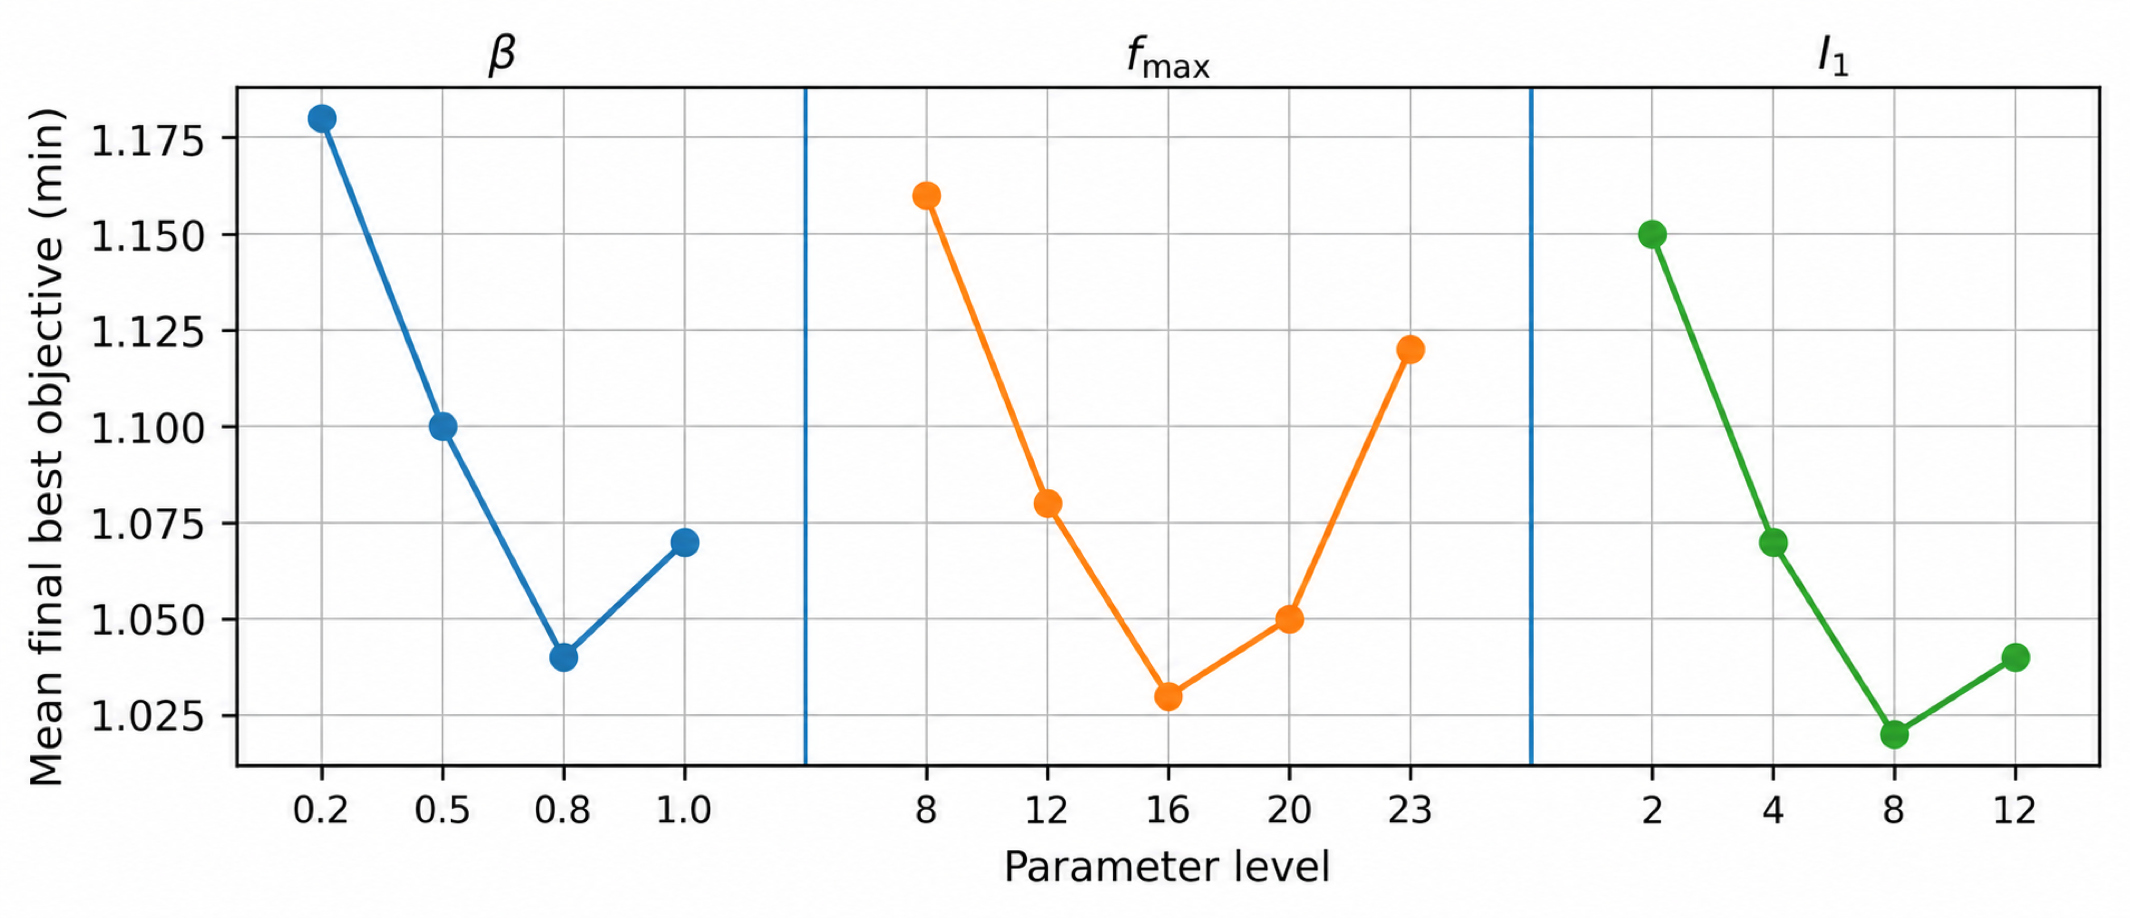
\includegraphics[width=0.95\linewidth]{bcseebo_main_effect.png}
  \caption{Main effect plot of BCS-EEBO hyperparameters (\(\beta\), \(f_{\max}\), and \(I_1\)).}
  \label{fig:main_effect_bcseebo}
\end{figure}

\subsection{Comparison with Other Algorithms}
\subsubsection{Global Modeling Performance}

Fig.~\ref{fig:rastrigin_global_modeling} compares the true objective-function surface of the two-dimensional (2D) Rastrigin function with the BCS-GP, BO-GP, and BCS-EEBO fused surrogate (Comb-GP). The global optimum is marked by a star. Figs.~\ref{fig:rastrigin_global_modeling}(b)--(d) show BCS-GP, BO-GP, and Comb-GP, respectively, for $M=25$ samples. Under this sparse design, BCS-GP uses the sparse DCT representation to recover global and oscillatory structure, whereas BO-GP with a Mat\'ern-$5/2$ kernel primarily models correlations supported by the observed samples and produces a smoother reconstruction. Comb-GP integrates the transform-domain information from BCS-GP with the local predictive information from BO-GP, yielding a more balanced reconstruction of the global trend and local variation.

At $M=90$, all three surrogate reconstructions improve; see Figs.~\ref{fig:rastrigin_global_modeling}(e)--(g). BCS-GP recovers more of the global oscillatory structure as additional measurements become available, while BO-GP captures finer variation around the sampled regions but retains the smoothing behavior induced by its stationary Mat\'ern-$5/2$ kernel. By combining these complementary estimates, Comb-GP more closely follows the true objective-function surface across both sampled and sparsely observed regions. These results show that surrogate-level fusion improves global reconstruction under sparse-to-moderate sampling on this multimodal, non-stationary example.

\begin{figure}[t]
  \centering
  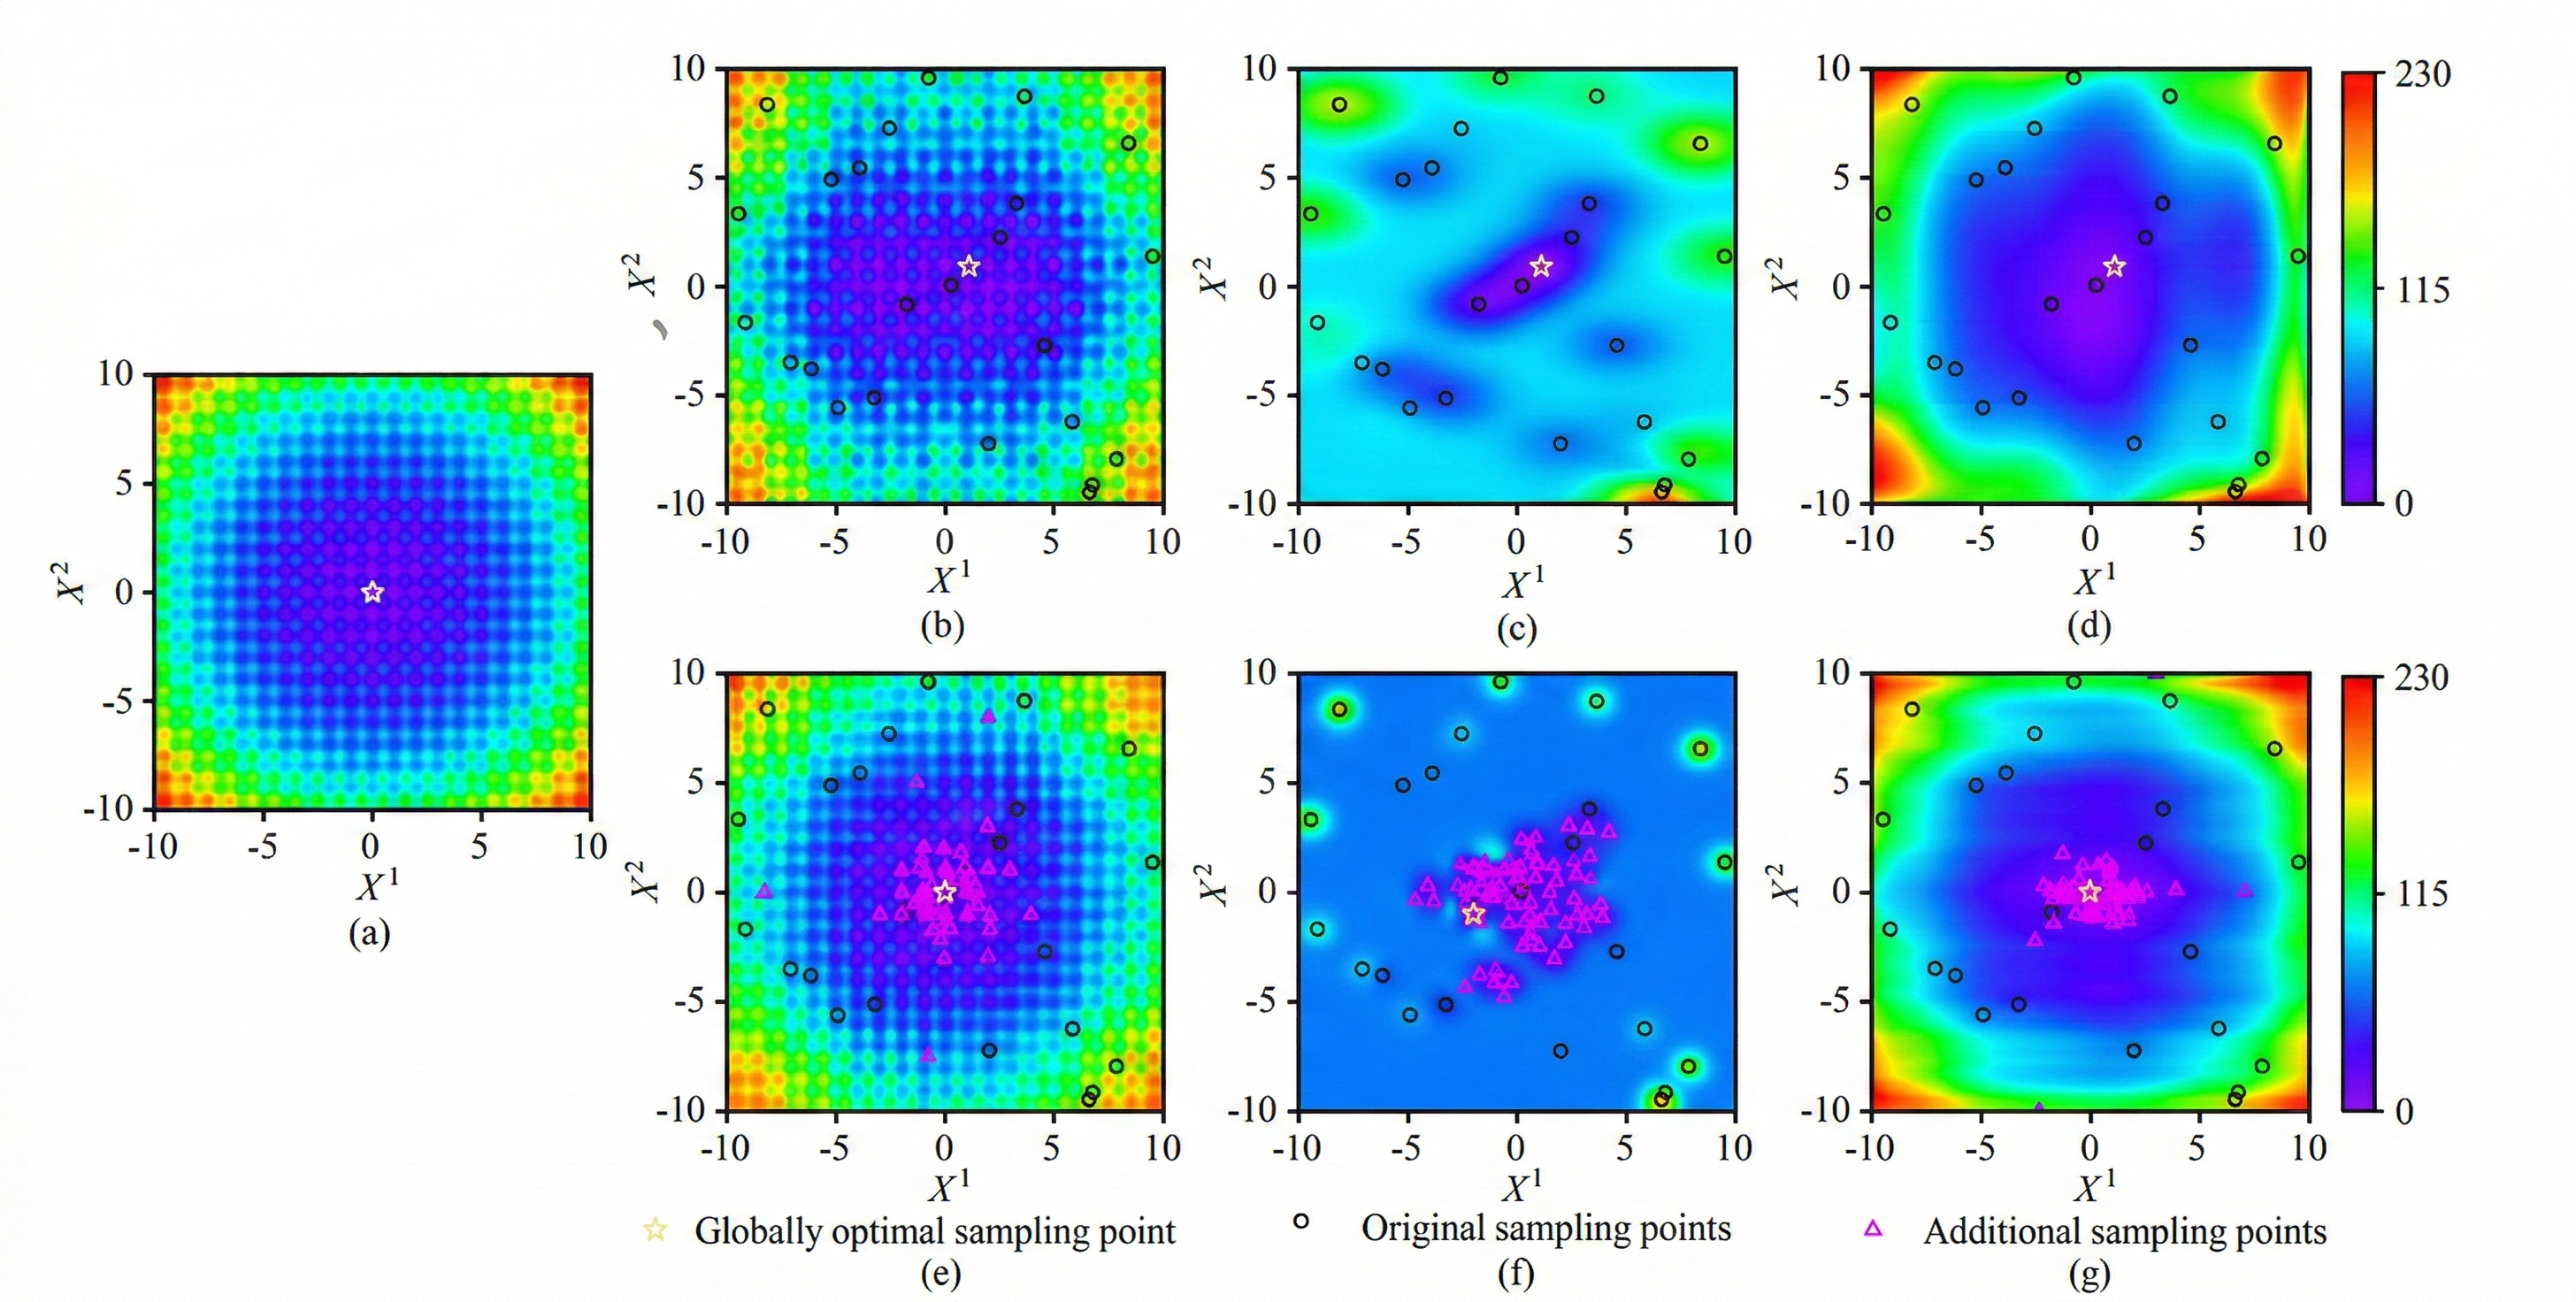
\includegraphics[width=0.98\linewidth]{demo_nonwatermark.png}
  \caption{Global modeling on the 2D Rastrigin function.
  (a) True objective-function surface.
  (b) BCS-GP with $M=25$ samples.
  (c) BO-GP with $M=25$ samples.
  (d) BCS-EEBO fused surrogate (Comb-GP) with $M=25$ samples.
  (e) BCS-GP with $M=90$ samples.
  (f) BO-GP with $M=90$ samples.
  (g) BCS-EEBO fused surrogate (Comb-GP) with $M=90$ samples.
  Color indicates the function value with a shared colorbar.
  Black dots denote sampled points and the star marks the global optimum at $(0,0)$.}
  \label{fig:rastrigin_global_modeling}
\end{figure}


\subsubsection{Batch Modeling Performance}
Surrogate accuracy and calibration are evaluated through batch active learning on noisy four-dimensional (4D) Sphere, Rosenbrock, Rastrigin, Ackley, and Griewank functions; see Fig.~\ref{fig:NLL}. Each method receives the same evaluation budget over four sequential batches. After each batch, the surrogate is refitted to all collected evaluations. Predictive calibration is measured by negative log-likelihood (NLL), and predictive accuracy is measured by root mean squared error (RMSE); lower values are better for both metrics. The curves report means and one-standard-error bands over repeated trials.

These benchmark functions cover complementary landscape characteristics commonly used to assess global optimization algorithms \cite{JamilYang2013}. The Sphere function is a smooth, convex, separable, and unimodal baseline, whereas the Rosenbrock function is nonseparable and contains a narrow, curved valley that makes progress toward its global minimum difficult \cite{Rosenbrock1960}. The Rastrigin function superimposes periodic oscillations on a quadratic envelope and therefore contains many regularly distributed local minima. The Ackley function combines an almost flat outer region with a narrow central basin and numerous local minima \cite{Ackley1987}. The Griewank function combines a quadratic trend with a multiplicative cosine term, producing widespread local minima and variable interactions \cite{Griewank1981}. Together, the five functions test surrogate reconstruction from a simple smooth response to curved, oscillatory, and strongly multimodal landscapes.

The comparison set spans distinct probabilistic surrogate families. GP-TS uses a conventional GP posterior and Thompson sampling to draw surrogate functions and select promising queries \cite{HernandezLobato2017PDTS}. BART-BO replaces the GP with Bayesian additive regression trees, whose posterior ensemble of regression trees can adapt to nonlinear interactions and local changes in the response structure \cite{Chipman2010BART,Lei2021AdaptiveBO}. Deep Networks for Global Optimization (DNGO) learns nonlinear basis functions with a deep neural network and places a Bayesian linear model on the resulting features to provide predictive uncertainty \cite{Snoek2015DNGO}. TP-BO instead uses a Student-$t$ process surrogate, whose heavy-tailed predictive distribution and data-dependent predictive covariance provide a flexible alternative to a GP \cite{Shah2014StudentTProcess}. These baselines therefore compare BCS-EEBO with GP, Bayesian-tree, neural-feature, and heavy-tailed process surrogates under the same batch budget.

As shown in Fig.~\ref{fig:NLL}, BCS-EEBO attains low NLL and RMSE across the tested functions and improves as additional batches are collected. The largest differences occur on the multimodal Rastrigin, Ackley, and Griewank functions, where global oscillatory and non-stationary structure affects uncertainty-guided sampling. The relative-rank panels place BCS-EEBO among the top-performing methods on both metrics across functions and batches. Compared with GP-TS, BART-BO, DNGO, and TP-BO, BCS-EEBO is especially competitive on the multimodal functions and shows steady improvement as additional batches are collected. The results associate the two-level fusion with more informative sampling and greater surrogate fidelity under noisy, evaluation-limited conditions.
\begin{figure}[t]
  \centering
  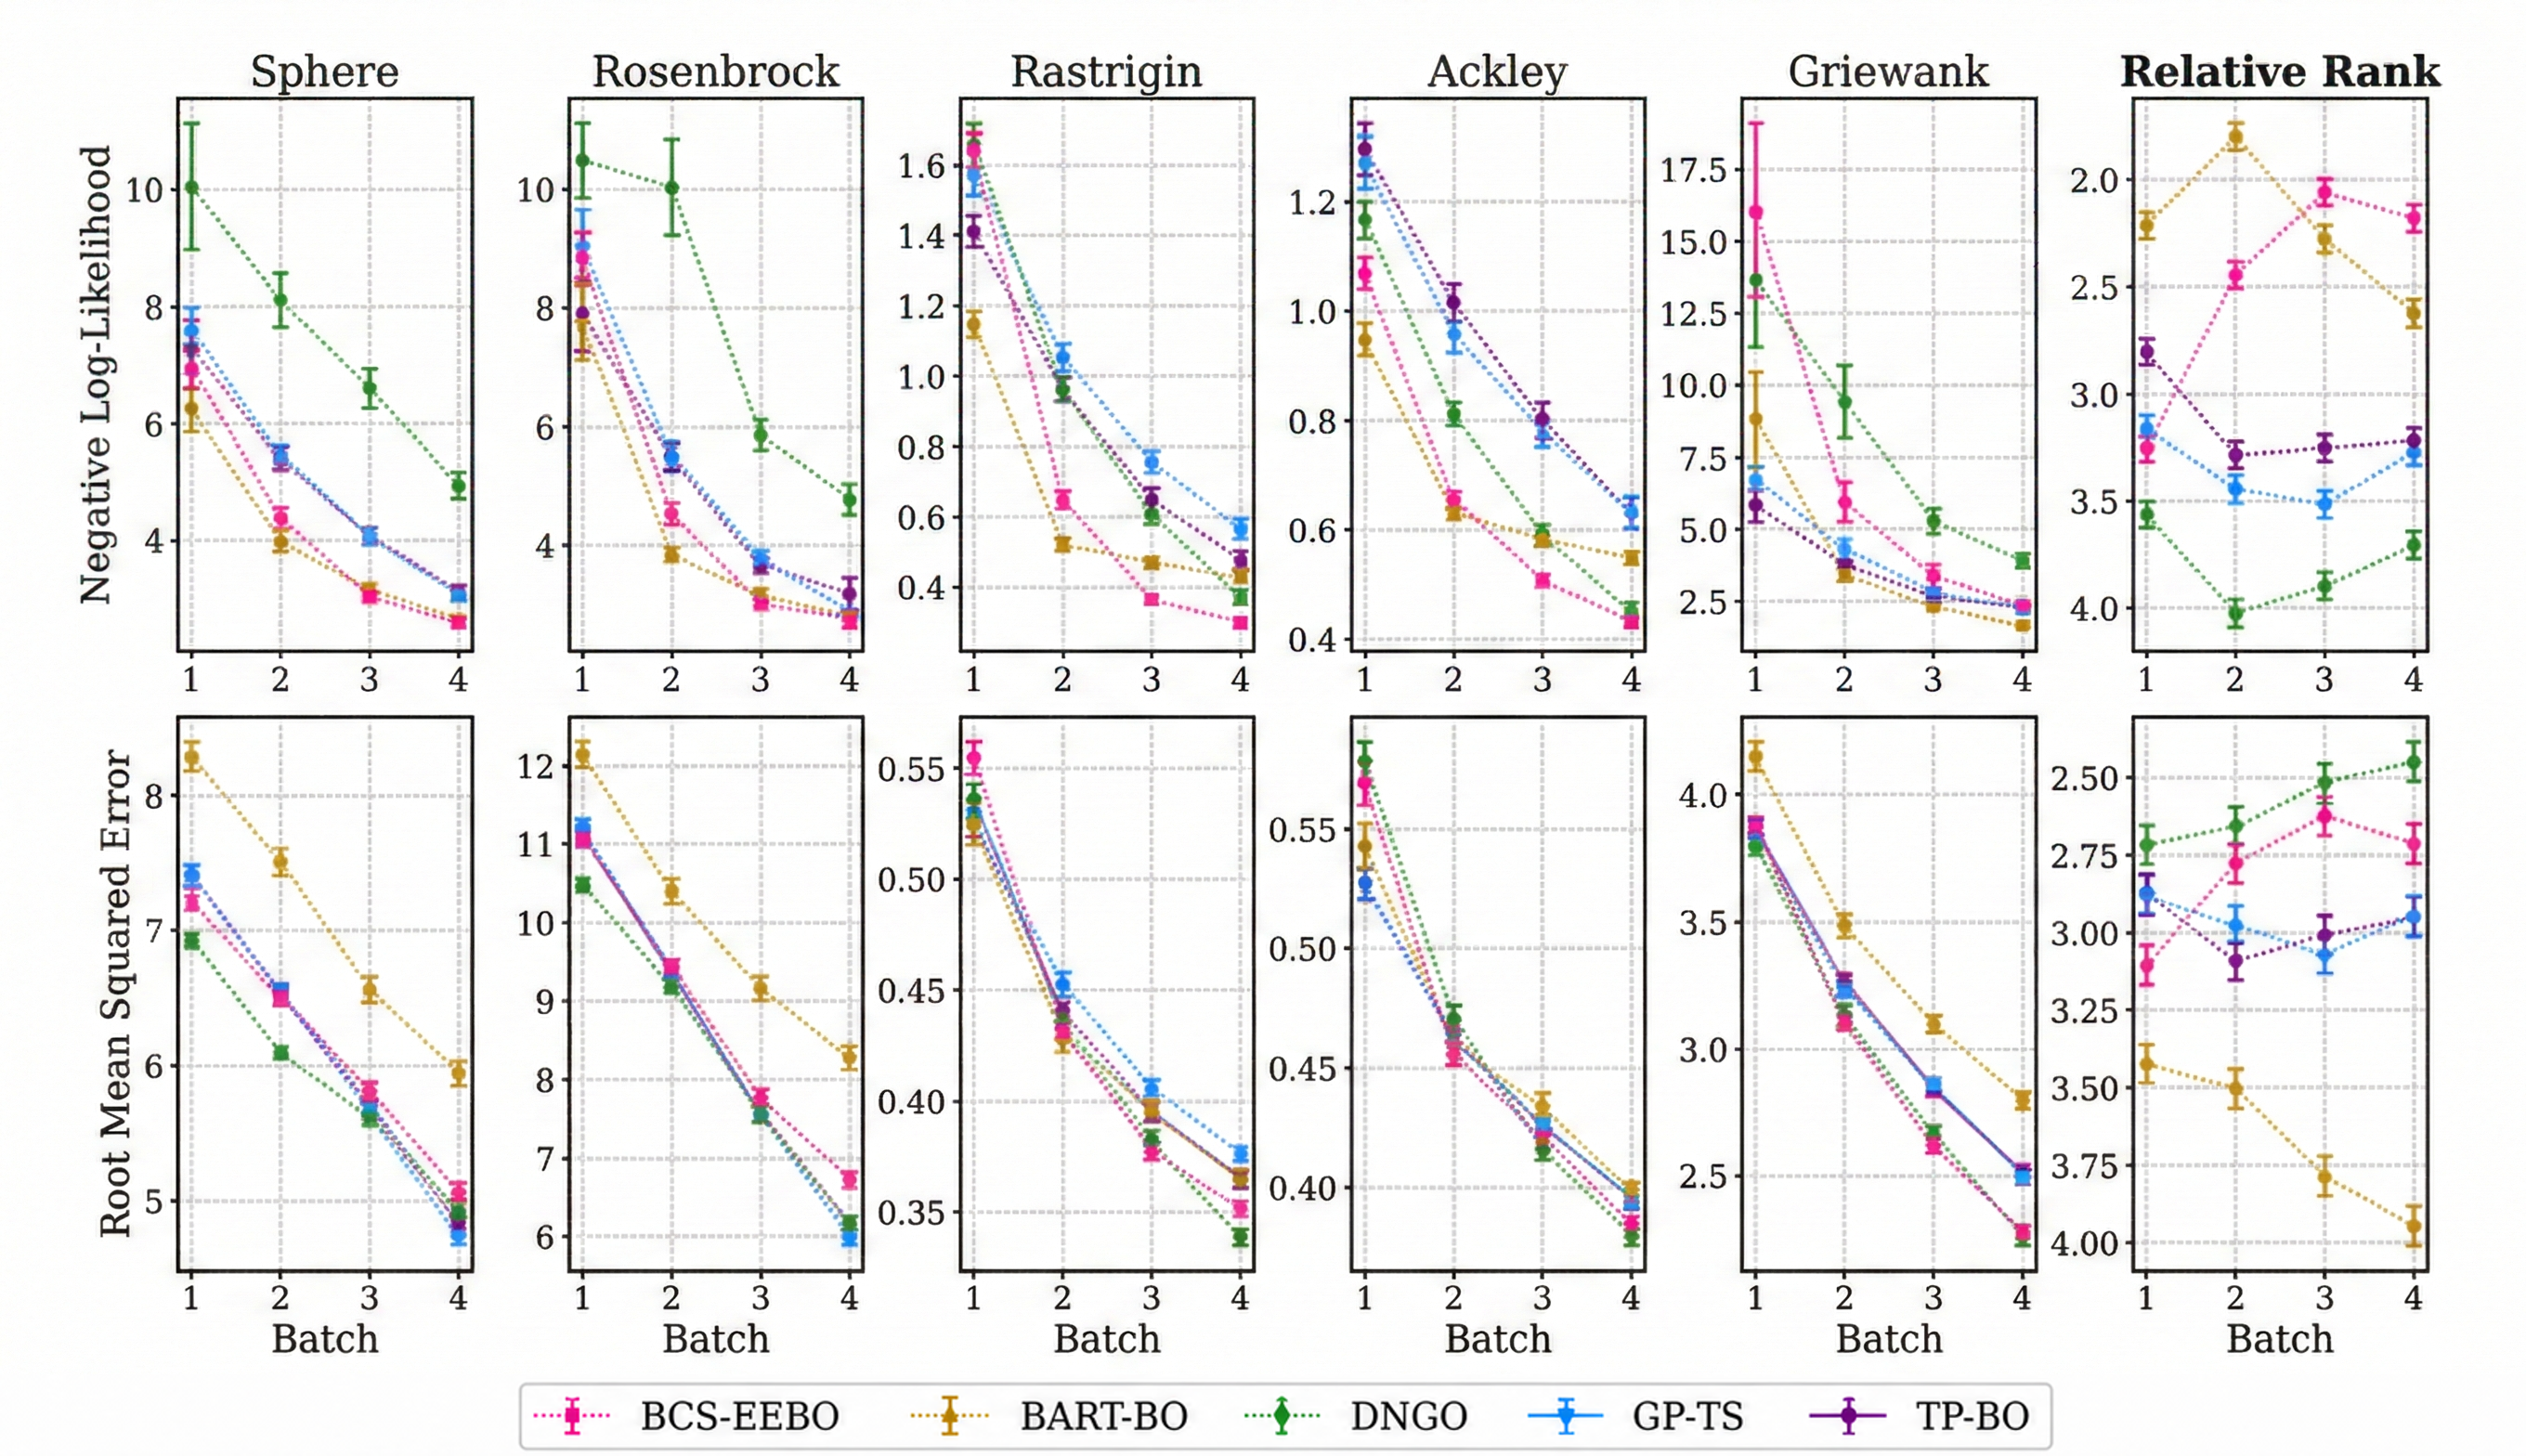
\includegraphics[width=0.98\linewidth]{NLL.png}
  \caption{Model accuracy in batch active learning. NLL and RMSE are reported over four batches of $q=16$ evaluations across 30 independent runs. BCS-EEBO ranks among the top two methods on both metrics.}
  \label{fig:NLL}
\end{figure}

\subsubsection{Noisy Synthetic Test Functions}
\label{subsec:noisy_synthetic}

BCS-EEBO is next evaluated on noisy synthetic functions under a two-shot batch-BO budget. The protocol uses $B=2$ batches with $q=24$ evaluations per batch. The first group contains the five-dimensional (5D) Sphere, Rosenbrock, Rastrigin, Ackley, and Griewank functions, covering unimodal and multimodal landscapes. Observation noise is added to every task. As shown in Fig.~\ref{fig:optimization_demo}, BCS-EEBO attains the best or second-best performance under the common budget, with the largest gains on Rastrigin, Ackley, and Griewank.

The second group contains the 5D Schwefel, Step, Quartic, Alpine 1, and L\'evy functions, which introduce discontinuities, heavy-tailed behavior, or local irregularities; see Fig.~\ref{fig:optimization_demo_2}. BCS-EEBO maintains a favorable relative rank across these tasks. The differences are largest for functions with pronounced global oscillations or irregular local structure, consistent with the use of transform-domain uncertainty and surrogate fusion.

\begin{figure*}[t]
  \centering
  % NOTE(rank-sync): Fig. 5 group end ranks are 1.10, 2.00, 4.20, 4.30, 3.40.
  % Their elementwise mean with the Fig. 6 ranks equals the pooled Fig. 7 ranks.
  % TODO(real-data): Regenerate these ranks from the final experimental logs.
  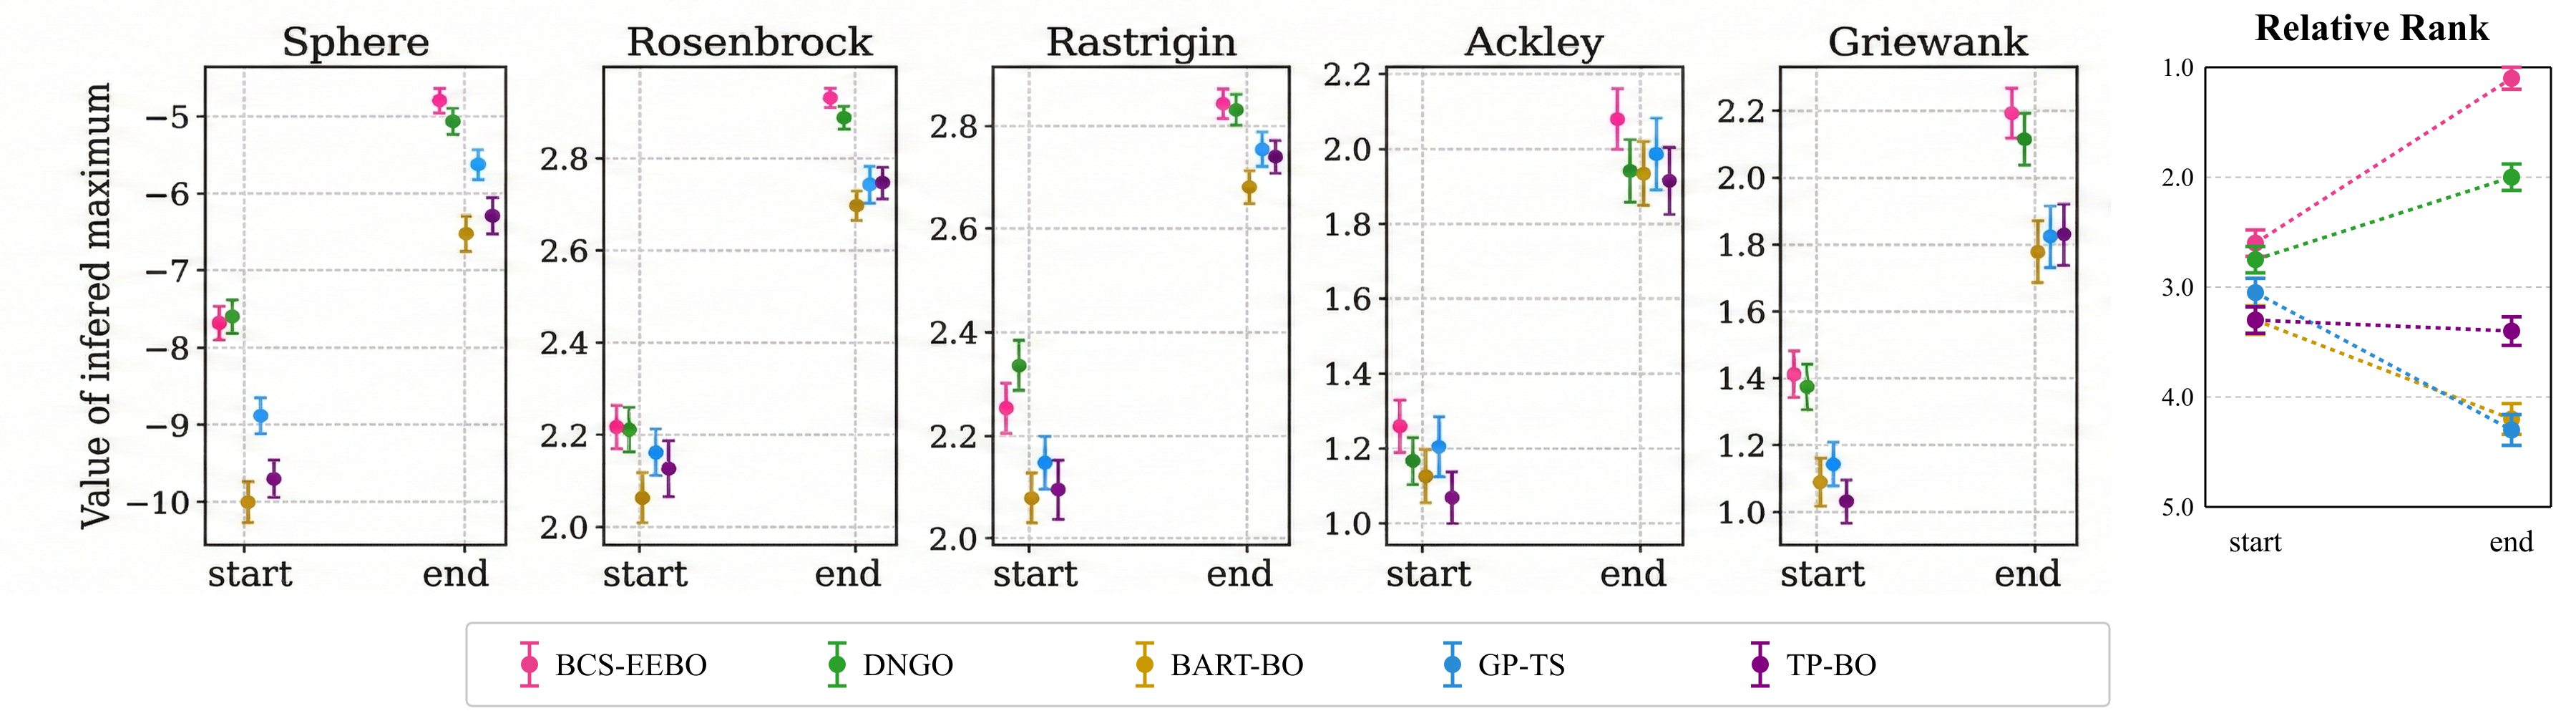
\includegraphics[width=\textwidth]{compare_1V2.png}
  \caption{Out-of-sample optimization performance on noisy $5$D synthetic benchmark functions. Panels correspond to Sphere (5D), Rosenbrock (5D), Rastrigin (5D), Ackley (5D), and Griewank (5D). The final panel shows the relative-rank summary for this five-function group; its pooled mean with the Fig.~\ref{fig:optimization_demo_2} ranks is reported in Fig.~\ref{fig:friedman_bd}. Markers and error bars summarize 30 independent runs; the relative ranks are computed from the function-level median final-best values defined in Sec.~\ref{subsec:nonparametric_tests}.}
  %(see Sec.~\ref{subsec:experimental_setup}).}
  \label{fig:optimization_demo}
\end{figure*}

\begin{figure*}[t]
  \centering
  % NOTE(rank-sync): Fig. 6 group end ranks are 1.30, 2.60, 3.60, 4.10, 3.40.
  % Their elementwise mean with the Fig. 5 ranks is 1.20, 2.30, 3.90, 4.20, 3.40.
  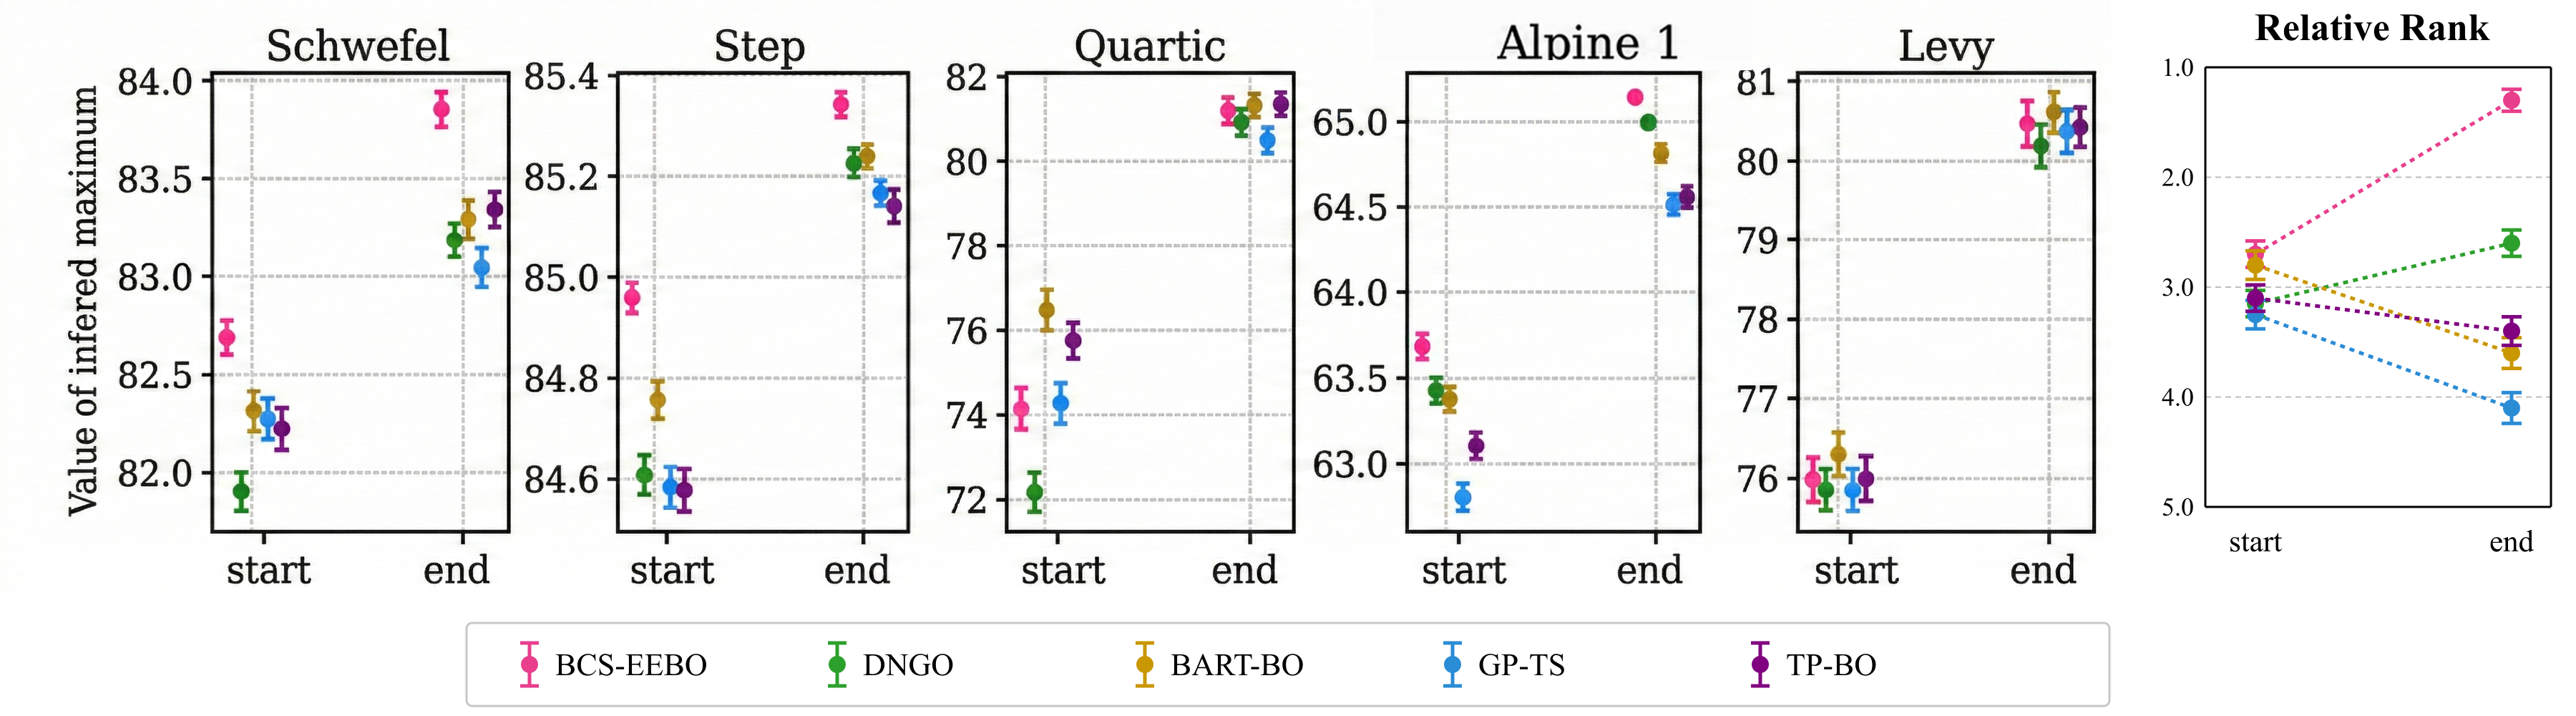
\includegraphics[width=\textwidth]{compare_2.png}
  \caption{Out-of-sample optimization performance on noisy $5$D synthetic benchmark functions. Panels correspond to Schwefel (5D), Step (5D), Quartic (5D), Alpine 1 (5D), and L\'evy (5D). The final panel shows the relative-rank summary for this five-function group; its pooled mean with the Fig.~\ref{fig:optimization_demo} ranks is reported in Fig.~\ref{fig:friedman_bd}. Markers and error bars summarize 30 independent runs; the relative ranks are computed from the function-level median final-best values defined in Sec.~\ref{subsec:nonparametric_tests}.}
  \label{fig:optimization_demo_2}
\end{figure*}

\subsection{Nonparametric Statistical Analysis}
\label{subsec:nonparametric_tests}

% TODO(real-data): The numerical results in this subsection, Fig.~\ref{fig:friedman_bd},
% and Table~\ref{tab:friedman_wilcoxon} are draft values. Recompute them from
% the original independent-run logs before manuscript submission. Verify that
% every algorithm--function combination contains exactly 30 valid runs.
The ten benchmark functions in Figs.~\ref{fig:optimization_demo} and~\ref{fig:optimization_demo_2} are analyzed jointly. For each algorithm--function combination, the median final-best objective value over 30 independent runs is used as the function-level performance measure. After orienting all measures so that larger values indicate better performance, the five algorithms are ranked separately on each function, with rank 1 assigned to the best-performing method and average ranks used for ties. The resulting $10\times5$ rank matrix is analyzed using the Friedman test, treating the benchmark functions as blocks ($N=10$) and the algorithms as treatments ($k=5$).

First, the Friedman test is used as an omnibus nonparametric test of the null hypothesis that there is no systematic performance difference among the algorithms and, consequently, that their expected ranks are equal \cite{Friedman1937,Demsar2006}. Let $\bar{R}_j$ denote the average rank of algorithm $j$. In the absence of ties, the Friedman statistic is
\begin{equation}
\chi_F^2=\frac{12N}{k(k+1)}
\left[\sum_{j=1}^{k}\bar{R}_j^2-\frac{k(k+1)^2}{4}\right].
\label{eq:friedman_test}
\end{equation}
The standard tie correction is applied if tied ranks occur within a function. Across the ten functions, the Friedman test gives $\chi_F^2(4)=24.56$ with $p=6.17\times10^{-5}$. The null hypothesis is therefore rejected at $\alpha=0.05$, providing evidence of an overall difference among the algorithms. This omnibus result does not, by itself, identify which algorithms differ.
% TODO(real-data): Recompute the Friedman statistic with the standard tie
% correction if the final function-level summaries contain any ties.

Because the omnibus test is significant, BCS-EEBO is used as the control algorithm in a Bonferroni--Dunn post-hoc analysis \cite{Dunn1961,Demsar2006}. The critical difference (CD) is
\begin{equation}
\mathrm{CD}_{\alpha}=q_{\alpha}
\sqrt{\frac{k(k+1)}{6N}},
\label{eq:bonferroni_dunn_cd}
\end{equation}
where $q_{\alpha}=z_{1-\alpha/[2(k-1)]}$ is the two-sided Bonferroni-adjusted normal critical value for the $k-1$ comparisons with the control. A control comparison is significant when $|\bar{R}_j-\bar{R}_{\mathrm{BCS\text{-}EEBO}}|>\mathrm{CD}_{\alpha}$. For $k=5$ and $N=10$, $\mathrm{CD}_{0.05}=1.766$ and $\mathrm{CD}_{0.10}=1.585$. Because BCS-EEBO has the smallest average rank in the present results, Fig.~\ref{fig:friedman_bd} displays the corresponding upper thresholds, $\bar{R}_{\mathrm{BCS\text{-}EEBO}}+\mathrm{CD}_{\alpha}$, as solid and dashed horizontal lines. BART-BO, GP-TS, and TP-BO exceed the $\alpha=0.05$ threshold of $1.20+1.766=2.966$, whereas DNGO does not.

\begin{figure}[t]
  \centering
  % Single-column statistical figure; ranks match the last panels of Figs.~5--6.
  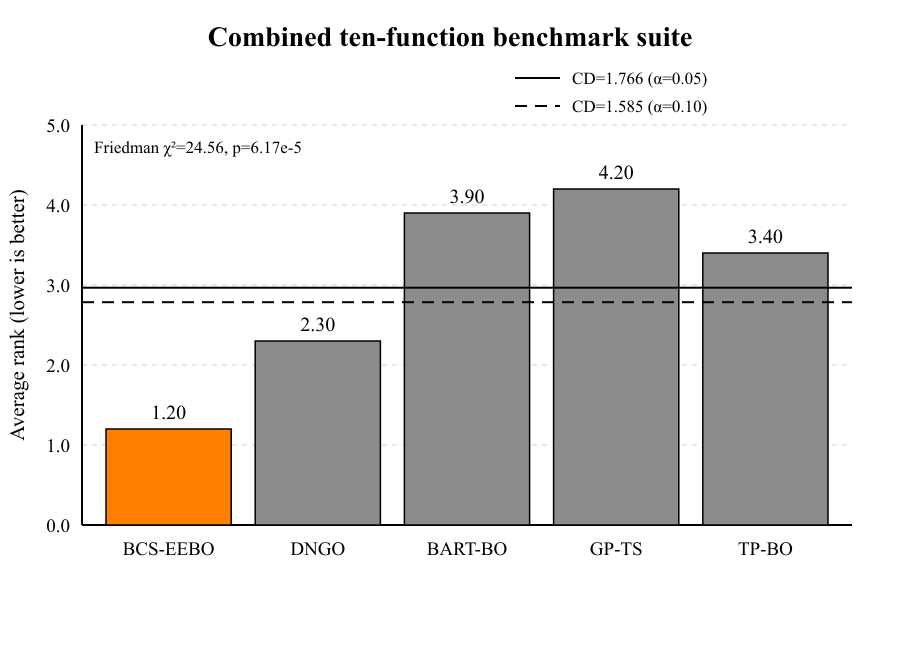
\includegraphics[width=\linewidth]{friedman_bonferroni_dunn.png}
  \caption{Friedman average ranks and Bonferroni--Dunn control-comparison results for the combined ten-function benchmark suite in Figs.~\ref{fig:optimization_demo} and~\ref{fig:optimization_demo_2}. Lower average ranks are better. The solid and dashed lines denote the BCS-EEBO average rank plus the critical difference at $\alpha=0.05$ and $\alpha=0.10$, respectively.}
  \label{fig:friedman_bd}
\end{figure}

As a complementary pairwise analysis, a two-sided Wilcoxon signed-rank test compares BCS-EEBO with each alternative using one matched pair per benchmark function \cite{Wilcoxon1945}. Each pair consists of the two algorithms' function-level summaries on the same test function. Before this analysis, the summaries are standardized within each function on a common higher-is-better scale so that differences in the numerical ranges of the benchmark functions do not determine the signed ranks. To control the family-wise error rate across the $k-1=4$ control comparisons, the raw $p$-values are Bonferroni-adjusted as $p_{\mathrm{adj}}=\min[(k-1)p,1]$, and significance is assessed at $p_{\mathrm{adj}}<0.05$. A competitor is labeled significantly worse only when the adjusted test is significant and its paired performance is lower than that of BCS-EEBO. The adjusted test does not distinguish DNGO from BCS-EEBO ($p_{\mathrm{adj}}=0.336$), whereas BART-BO, GP-TS, and TP-BO are significantly worse ($p_{\mathrm{adj}}=0.008$), consistent with the Bonferroni--Dunn result. The BCS-EEBO row in Table~\ref{tab:friedman_wilcoxon} is marked with a dash because no self-comparison is performed.
% TODO(real-data): Replace the draft standardized scores with function-level
% medians computed from the logs and document the exact function-wise
% standardization used before the Wilcoxon signed-rank tests.


\begin{table}[t]
  \centering
  \caption{Friedman average ranks and Bonferroni-adjusted Wilcoxon test results.}
  \label{tab:friedman_wilcoxon}
  \footnotesize
  \renewcommand{\arraystretch}{1.12}
  \begin{tabular*}{\columnwidth}{@{\extracolsep{\fill}}lccc@{}}
  \hline
  & \textbf{Friedman} &
  \multicolumn{2}{c}{\textbf{Wilcoxon vs. BCS-EEBO}} \\
  \cline{2-4}
  \textbf{Algorithm} &
  \textbf{Avg. rank} &
  \textbf{Adjusted $p$-value} &
  \textbf{Reject $H_0$?} \\
  \hline
  \textbf{BCS-EEBO} & \textbf{1.200} & --    & --  \\
  DNGO              & 2.300          & 0.336 & No  \\
  BART-BO           & 3.900          & 0.008 & Yes \\
  GP-TS             & 4.200          & 0.008 & Yes \\
  TP-BO             & 3.400          & 0.008 & Yes \\
  \hline
  \end{tabular*}
  \vspace{2pt}

  \parbox{\columnwidth}{\scriptsize\raggedright
  \emph{Note:} For each Wilcoxon comparison, $H_0$ states that the paired function-level performance differences between BCS-EEBO and the comparison algorithm have a distribution symmetric about zero. Reported $p$-values are Bonferroni-adjusted.\par}
  \end{table}

\subsection{Ablation Experiments}
Table~\ref{tab:ablation} reports an ablation study of BCS-EEBO against the standard GP+EI baseline.
Overall, the full method achieves the best performance on both metrics, attaining the highest final best objective value (Max) and the lowest NLL. This indicates that the proposed design improves both the optimization outcome and the calibration of the surrogate predictive distribution.

Removing the BCS-driven acquisition term (\emph{without BCS acquisition}) decreases Max from $0.942$ to $0.913$, while NLL increases from $0.958$ to $1.004$. The covariance-based exploration signal therefore contributes information beyond EI alone.
Removing EI and retaining only the BCS acquisition (\emph{without EI}) produces a larger reduction in Max to $0.887$, although NLL remains relatively low at $0.992$. Without EI, uncertainty-direction exploration dominates the search; this improves model fit in some regions but slows refinement near the optimum.

BCS-GP+EI, which omits both surrogate-level fusion and the BCS acquisition term, improves on GP+EI with Max $0.921$ and NLL $0.987$. Thus, the BCS-induced surrogate provides useful global structure under non-stationarity. The performance gap to full BCS-EEBO confirms that the two fusion levels play complementary roles.

\begin{table}[t]
\centering
\caption{Ablation study of BCS-EEBO.}
\label{tab:ablation}
\setlength{\tabcolsep}{4.5pt}
\begin{tabular}{lcc}
\hline
\textbf{Method} & \textbf{Max} $\uparrow$ & \textbf{NLL} $\downarrow$ \\
\hline
GP + EI (Baseline) & $0.861 \pm 0.041$ & $1.327 \pm 0.073$ \\
\textbf{BCS-EEBO (Full)} & $\mathbf{0.942 \pm 0.028}$ & $\mathbf{0.958 \pm 0.052}$ \\
Without BCS acquisition  & $0.913 \pm 0.031$ & $1.004 \pm 0.056$ \\
Without EI (BCS acquisition only) & $0.887 \pm 0.038$ & $0.992 \pm 0.061$ \\
BCS-GP + EI  & $0.921 \pm 0.030$ & $0.987 \pm 0.055$ \\
\hline
\end{tabular}
\end{table}

\section{Conclusion and Future Work}
\label{sec:conclusion}

Expensive black-box global optimization under strong non-stationarity and limited evaluation budgets was studied. The proposed BCS-EEBO method combines a locally adaptive BO-GP with a BCS-induced predictor constructed from a sparse truncated DCT representation. At the acquisition level, EI is combined with an exploration score derived from the dominant uncertainty direction of the BCS posterior covariance. The resulting optimizer uses local predictive information while retaining exploration guided by transform-domain uncertainty.

On the 2D Rastrigin example, BCS-EEBO produces more accurate global reconstructions under sparse-to-moderate sampling. The ablation study attributes improvements in predictive calibration to surrogate-level fusion and improved exploration to the acquisition-level BCS term. Together, the results show that the two fusion levels address different aspects of non-stationary expensive optimization.

Several limitations remain. The truncated DCT dictionary restricts the represented structures; wavelets, learned overcomplete bases, and multiresolution dictionaries offer alternatives for other non-stationary patterns. The current surrogate and acquisition weights are heuristic, and principled online or decision-theoretic calibration remains an open problem. Extension to higher-dimensional continuous domains requires more efficient candidate generation and acquisition maximization, for example through constrained local search, trust regions, or latent subspaces. Constraints, multi-fidelity evaluations, and multiple objectives are not addressed in the present formulation. Regret and convergence analysis under model mismatch and non-stationary objectives also remains open.

\bibliographystyle{IEEEtran}
\bibliography{name}

\end{document}